\documentclass[a4paper,12pt,twocolumn]{article}
\usepackage[top=1in,bottom=1in,left=1in,right=1in]{geometry}
\usepackage[T1]{fontenc}
\usepackage[utf8]{inputenc}
%\usepackage{newunicodechar}
%\usepackage{lmodern}
\usepackage{textgreek}
\usepackage{amsmath}
\usepackage{mathtools}
\usepackage{graphicx}
\usepackage{float}
\usepackage[format=plain,labelfont={bf,it},font=it]{caption}
\usepackage{enumitem}
\usepackage{lipsum}
\usepackage{listings}
\usepackage{pdflscape}


\usepackage{tabularx}
%\usepackage{blindtext}
\usepackage{hyperref}
%\usepackage{pgfgantt}
\usepackage{setspace}
\usepackage{subcaption}
\usepackage{tikz}
\usepackage{chngcntr}
\usepackage{longtable}
\usepackage{xcolor,colortbl}
\usepackage{multicol} 
%\usepackage{mdframed} 
\usepackage{oubraces}
\usepackage{stfloats}
%\usepackage{fixltx2e}

\setcounter{tocdepth}{3}
\counterwithin{figure}{subsection}
\counterwithin{table}{subsection}

\usepackage[backend=bibtex,style=numeric,sorting=none]{biblatex}
\addbibresource{references.bib}
\renewcommand*{\bibfont}{\footnotesize}

% Our base colours
\definecolor{c1}{HTML}{ff7568} 
\definecolor{c2}{HTML}{8cbfff} 
\definecolor{c3}{HTML}{a6ddb7} 
\definecolor{darkred}{rgb}{0.6,0,0}

\lstdefinelanguage{asm}{
	morekeywords={ADC,ADD,ADDC,ADDI,ALU0,ALU1,AND,ANDI,BEQ,BGE,BGT,BR0,BR1,BRZ,BZ,CALL,CI0,CI1,CI2,CLC,CLN,CLS,COM,COMA,COMD,CPY0,CPY1,CPY2,CPY3,DEC,DIV,EQ,GE,GETAH,GETIF,GT,INC,INTRE,JUMP,LE,LT,LWHI,LWLO,MEM0,MEM1,MEM2,MEMHI,MEMLO,MOD,MOVE,MUL,MULHI,MULLO,NE,NULL,OR,ORI,PC0,PC1,POP,PUSH,RBWI,REG0,REG1,RET,RETI,RJUMP,ROL,ROR,SBC,SETC,SETI,SETN,SETS,SLL,SRA,SRL,SSETN,SSETS,STACK,STPT0,STPT1,SUB,SUBC,SUBI,SWHI,SWLO,XOR,XORI},
	sensitive=false,
	morecomment=[l]{;},
	morestring=[b]",
}
\lstset{language=asm, basicstyle=\ttfamily, commentstyle=\color{gray}, emphstyle={\color{darkred}}}

% This enviroment ensures that structures like listing and tables are not broken between columns or pages.
\newenvironment{blockpage}
{\begin{center}\begin{minipage}[c]{\linewidth}}
{\end{minipage}\end{center}}

% This allows placing figure in column
\newenvironment{colfigure}
{\par\medskip\noindent\minipage{\linewidth}}
{\endminipage\par\medskip}

\begin{document}
	
	\begin{titlepage}
		\newcommand{\HRule}{\rule{\linewidth}{0.5mm}}
		\begin{tikzpicture}[remember picture, overlay]
		\node [anchor=north east, inner sep=0pt]  at (current page.north east)
		{
\includegraphics[width=21cm]{../resources/graphics/ucl-banner-dl-port-outline.eps}};
		\end{tikzpicture}\\[3cm]
		\center
		
		\textsc{\Large University College London}\\[0.5cm]
		\textsc{\large Department of Electronic and Electrical Engineering}\\[0.5cm]
		
		\HRule \\[0.4cm]
		\setstretch{1.5}
		{ \huge \bfseries Performance characterisation of 8-bit RISC and OISC architectures}\\[0.4cm]
		\setstretch{1.0}
		\HRule \\[1.0cm]
		
		\begin{multicols}{3}
			
			\Large \emph{Author:}\\
			Mindaugas \textsc{Jarmolovi\v{c}ius}\\
			\href{mailto:zceemja@ucl.ac.uk}{zceemja@ucl.ac.uk}\\
			
			\columnbreak
			
			\Large \emph{Supervisor:}\\
			Prof. Robert \textsc{Killey}\\
			\href{mailto:r.killey@ucl.ac.uk}{r.killey@ucl.ac.uk}
			
			\columnbreak
			
			\Large \emph{Second Assessor:}\\
			Dr. Ed \\\textsc{Romans}\\
			\href{mailto:e.romans@ucl.ac.uk}{e.romans@ucl.ac.uk}
			
		\end{multicols}
		
		\vfill
		\setstretch{2.5}
		{ \large \bfseries A BEng Project Final Report}\\[1cm]
		\setstretch{1.0}
		{\large March 27, 2020}\\[2cm]
		
	\end{titlepage}
	
	\pagebreak
	\section*{Abstract}\label{sec:abstract}
	% !TeX root = index.tex
\iffalse
The abstract is written last and summarises the important points you are making in the report using one sentence for each point:

* What is the topic of the work? What is the goal?
* Why are you doing it? What are your motivations?
* Does this work appear in the literature and if so, what are you doing differently?
* What is the most significant result? Was it unexpected? What impact will it have?
\fi

One Instruction Set Computer (OISC), commonly implemented as Transport Triggered Architectures (TTAs) is a promising architecture that is successfully used in Application-Specific Instruction Set Processors (ASIPs) exploiting operation style parallelism, while keeping simplicity and flexibility. There is a lack of research in general purpose OISC with single data-instruction bus that could be used in lower power and performance comparable to an 8bit microcontroller using traditional Reduce Instruction Set Computer (RISC) architecture. This report describes the design, implementation and testing of two novel 8bit RISC and OISC-TTA processors, and investigates their characteristics and performance when implemented on FPGA. OISC required only a half of logic elements comparing to RISC, however it takes 71\% longer to execute designed benchmark, showing that OISC would need more than one data-instruction bus to outperform RISC.

	\vspace*{10cm}
	\tableofcontents
	\vfill\null\pagebreak
	
	
	\section{Introduction}\label{sec:introduction}
	% !TeX root = index.tex
\iffalse
The Introduction brings readers from a general understanding of the topic 
to a point where they can begin to understand what it is you are intending to do. 

It starts with broad statements and ends with specific statements about your project. 
Along the way it introduces readers to what has been done in the literature and 
then tells them why your project results will be different.

The Introduction provides a motivation for the work and tells readers what you will be telling them.
The following sections may be written simply as paragraphs; 
nothing more is really needed in the Introduction. 
You do not have to separate out each section.
The Funnel model is a good way to organise the Introduction.

1) The funnel model begins with a general statement about the general topical area;
 for example, “Antennas have been used for communications for at least 100 years”.
 It then narrows the focus repeatedly with further sentences by introducing work that has been 
 done in the literature with the appropriate citations.
 Finally, it reaches your project. By that time the reader knows in general terms what your work
 is about and understands your motivations. 
 The number of cited works ranges from a few to very many. 
 But whatever the number, they are the most significant in the field and have made the most impact on the historical development of the topic.

2) Your specific Aims and Objectives follow. Use bullet points for each and spend a few sentences describing each.

3) Follow your Aims and Objectives with a specific literature review. 
 In section 1, the review was rather broad. Now is the time to focus in on several journal articles 
 or products or activities that most closely match your own project work. 
 Use a few sentences to describe each one and show specifically what was useful about them. 
 Show how your work would improve on their work. You need only a few here. 
 Use those that are most similar and most like your project.

End the Introduction with a one-line description of the contents of each following Chapter.For example, “Chapter 2 focuses on.... Chapter 3 describes the work.... In Chapter 4, an outline of the measuring equipment ..., etc.”
\fi

Since the 70s there has been a rise of many processor architectures that try to fulfil specific performance and power application constraints. One of more notable cases are ARM RISC architecture being used in mobile devices instead of the more popular x86 CISC (Complex Instruction Set Computer) architecture in favour of simplicity, cost and lower power consumption \autocite{jamil_1995,blem_menon_sankaralingam_2013}. It has been shown that in low power applications, such as IoTs (Internet of Things), OISC implementation can be superior in power and data throughput compared to traditional RISC architectures \autocite{yokota_saso_hara-azumi_2017, ahmed_sakamoto_anderson_hara-azumi_2015}. This project proposes to compare two novel RISC and OISC 8bit architectures and compare their performance, design complexity and efficiency.


\subsection{Aims and Objectives}

The project has three main objectives:
\begin{enumerate}
	\item Design and build a RISC based processor.
	\item Design and build an OISC based processor. 
	\item Design and perform a fair benchmark on both processors. 
\end{enumerate}

Both processors must be Turing-Complete, meaning they are computationally universal and theoretically would be capable of emulating any other Turing-Complete machine if given enough time and resources.

\subsection{Related Work}
\label{subsec:supporting_theory}
This section goes through supporting theory of RISC and OISC architectures, and their comparison.

The principal functions of general OISC architecture should have advantage in performance and power consumption while having lower transistor count. There are several theoretical models to implement a processor using only a single instruction, most important models are subtract and branch, MOVE and half-adder architectures \autocite{gilreath_laplante_2003}. 

Some researches have proven benefits of the subtract and branch architecture over the RISC:\\
$\bullet$ Using an OISC \texttt{SUBLEQ} (SUBtract and jump if Less or EQual to zero) as a coprocessor for the Microprocessor without Interlocked Pipelined Stages - Instruction Set Architecture (MIPS-ISA) processor to emulate the functionality of different classes shows desirable area/performance/power trade-offs \autocite{ahmed_sakamoto_anderson_hara-azumi_2015}.\\
$\bullet$ Comparing an OISC \texttt{SUBLEQ} multicore to a RISC achieves better performance and lower energy for streaming data processing \autocite{yokota_saso_hara-azumi_2017}.

Looking at the OISC \texttt{MOVE} type, it has been researched since early 90s. It has been shown that the OISC \texttt{MOVE} can benefit from a VLIW (very large instruction word) arrangement, classifying it as a SIMO (single instruction, multiple operation) or a SIMT (single instruction, multiple transports) architectures. The problem with all of these arrangements is that they exhibit poor or complex hardware utilization. OISC \texttt{MOVE} has been proposed as a design framework enabling a lower complexity, better hardware utilization, and a scalable performance \autocite{5348869}. In this framework a TTA is proposed which describes how a single instruction should transport the data. To support theoretical benefits, a \texttt{MOVE32INT} TTA has been designed \autocite{Corporaal94move32int} and proven to be a superior architecture to the RISC. Using a 1.6$\mu m$ fabrication technology, RISC has achieved 20MHz clock with 20Mops/second, while \texttt{MOVE32INT} implemented using SoGs (Sea of Gates) achieved 80MHz with 320Mops/second \autocite{289981}.

The TTA framework was further used in other researches to implement ASIPs to solve various problems. Some relevant examples are RSA calculation \autocite{6128530}; matrix inversion \autocite{1540373}; Fast Fourier Transform (FFT) \autocite{8682289}; IWEP, RC4 and 3DES encryption \autocite{922340}; Parallel Finite Impulse Response (FIR) filter \autocite{1511285}; Low-Density Parity-Check (LDPC) encoding \autocite{6855236}; Software Defined Radio (SDR) \autocite{7363689}. One of the most recent researches uses TTA architecture to solve Compressive Sensing algorithms. Research showed 9 times higher energy efficiency to that of FPGA implemented NIOS II processor, and theoretical 20 time energy efficiency compared to that of ARM Cortex-A15 \autocite{8573494}. In this particular research however, the used ARM Cortex-A15 with 28nm Metal Gate CMOS technology was compared to a TTA implemented on Altera Cyclone IV FPGA with 60nm Silicon Gate CMOS technology. Both processor implementations cannot be directly compared.

Most of these researches show that TTA has a greater power efficiency, a higher clock frequency limit and a lower logic resource count. 

These benefits come with an expense, VLIW has bigger instruction word, therefore a bigger program size. TTA especially suffers from this due to the redundant instructions. Some proposed solutions are variable length instructions and instruction templates, which reduce program size by between 30\% and 44\% \autocite{1213033,6893206}; a compression based on arithmetic coding \autocite{4627144}; and a method to remove redundant instructions \autocite{5403730}. 
Software is another difficulty as the compiler needs to take additional steps for the data transportation optimisations. TTA software can be easily exploited however, to embed a software pipelining and parallelism without need of the extra hardware \autocite{4595596}.

With the proposed \texttt{MOVE} framework, hardware utilisation was shown to be improved by reducing transition activity \autocite{1207041}, reducing interconnects was shown to save 13\% of energy \autocite{6972455} on a small scale. A novel architecture named SynZEN also showed a further improvement by using an adaptable processing unit and a simple control logic \autocite{6403142}.

\subsection{Project contents}
Section \ref{sec:objectives} will provide more detail on the motivation and project decisions based on \nameref{subsec:supporting_theory}. Section \ref{sec:theory} explains theory and result predictions. Section \ref{sec:methods} explains both processor design choices and how each processor part is implemented on OISC and RISC processors. It also includes assembler design and system setup. In section \ref{sec:results}, results will be discussed, including benchmark methods and future work. Summary and conclusion of design and results can be found in section \ref{sec:conclusion}. Appendix in section \ref{sec:appendix} includes any other information, such as both processors' instruction sets.

	\vfill\pagebreak
	\section{Goals and Objectives}\label{sec:objectives}
	% !TeX root = index.tex
\iffalse
This chapter describes your Goals and Objectives. 
Indicate how your work is intended to expand on previous historical work.
Present your motivations; why are you doing this?
Indicate the type of project you have(see the list above).

Types of Projects:
2) Design and Construction projects:
These types of projects involve the design and construction of some 
electrical or electronic apparatus or device within the bounds 
of the department's educational mandate.
\fi


This project can be classified as a Design and Construction type, which explores alternative designs of a processor architecture and microarchitecture. Main goals are:
\begin{enumerate}
	\item Study and explore computer architectures, SystemVerilog and the assembly language. 
	\item Compare how well an OISC \texttt{MOVE} architecture would perform in a low performance microcontroller application comparing to equivalent and most commonly used RISC architecture.
	\item View an alternative method of using OISC \texttt{MOVE} in a SISO (single instruction, single operation) structure, comparing to more commonly implemented TTAs VLIW architectures that are either a SIMO or a SIMT structure.
\end{enumerate}



\subsection{RISC Processor}
The RISC architecture will be mainly based on MIPS architecture explained in \autocite{harris_harris_2013}, except it this RISC processor would have 8bit data bus, four general purpose registers and would have multiple optimisations related to 8bit limits. Some of minimalistic design ideas was also from \autocite{gilreath_laplante_2003}.


\subsection{OISC Processor}
OISC \texttt{MOVE} has many benefits from VLIW and SIMO or SIMT design, however there is a lack of research investigating and comparing more general purpose OISC \texttt{MOVE} 8bit processor with a short instruction word and a SISO configuration. The main theory for building OISC architecture will be based on \autocite{gilreath_laplante_2003}.

\subsection{Design Criteria}
In order to fairly comparison between both architectures, a common design criteria is set:
\begin{description}
	\item[$\bullet$] Minimal instruction size
	\item[$\bullet$] Minimalistic design
	\item[$\bullet$] 8bit data bus width
	\item[$\bullet$] 16bit ROM address width
	\item[$\bullet$] 24bit RAM address width
	\item[$\bullet$] 16bit RAM word size
\end{description}
When constructing these points, time and equipment resources were taken into the consideration. 

\subsection{Benchmark}
This benchmark includes different algorithms that are commonly used in 8bit microcontrollers, IoT devices or similar low power microprocessor applications.


\iffalse
This is just a list of research papers and relative context:
\autocite{5936440} - Novel processor for Multiple Instruction Multiple Data packet triggered architecture for pipeline and parallel processing.


\autocite{7363689} - Implementing TTA for SDR and focuses on power optimisations. It show ~24.8-26.1\% decrease in power consumption with 3.3\% area increase.
\autocite{1511285} - Scalable FIR filtering on TTA
\autocite{289981} - MOVE32INT TTA implementation. Achieved parallel processing with 80MHz 320Mops/s comparing to RISC 20MHz 20Mops/s. Includes automated design
\autocite{6855236} - Parallel programming of a TTA for LDPC encoding application
\autocite{922340} - TTA for encryption specific ASIP
\autocite{8682289} - Low power implementation TTA for FFT
\autocite{6128530} - Implemented TTA that is efficent on RSA calculations, 3 1024bit pairs/s at 100MHz
\autocite{1540373} - ASIP TTA for matrix inversion.
\autocite{6403142} - A novel microachitecture that combines VLIW and TTA for different applications. Takes less area than existing TTA and VLIW
\autocite{8573494} - Compressive Sensing Applications on ARM Cortex-A15, NIOS II and TTA architectures. TTA has lowest time and power consumption, however about 2.5 higher area to NIOS II

\autocite{840031}  - Introduce Test space exploration costs for TTA templates.


\autocite{4595596} - Focuses on software pipelining and solved with GNU Linear Programming Kit (Very interesting)
\autocite{8425389} - Using soft cores in comparision to VLIW to have 67\% of resources with up to 88\% improvement in execution time and 21-49\% cost in program size.


\autocite{5403730} - TTA instruction redundancy remoal method with base plus offset addressing load/store function unit (LSFU)
\autocite{6972455} - Reducing VLIW interconnects to achieve 10\% core energy in 4-issue VLIW
\autocite{1207041} - Try to reduce power by encoding buses thus reducing switching (read a bit more)
\autocite{4627144} - TTA code compression using arithmetic coding
\autocite{1213033} - Another template based compression method to improve code density
\autocite{6893206} - Instruction template based compression method for TTA processors
\fi

	\section{Theory and Analytical Bases}\label{sec:theory}
	\iffalse
This chapter presents the background physical or electrical theory
and on any analytical methods you will use to accomplish your goals.
If you have a research question, what is it?
Have you made any deductions from it that you are now testing?
What mathematical bases must be understood in order to interpret your results in Chapter 5?
Give the reader a solid understanding of the foundations here.
\fi


\textbf{Decided design criteria:}
\begin{description}
	\item[$\bullet$] Minimal instruction size
	\item[$\bullet$] Minimalistic design
\end{description}
	\vfill\pagebreak
	
	\section{Technical Method}\label{sec:methods}
	% !TeX root = index.tex
\iffalse
This chapter lays out your approach. 
What did you actually do to reach your goal, or attempt to reach your goal? 
What equipment did you use? 
How did you build the device? 
How did you set up the simulation: what mesh values, for example, did you use?

Provide enough detail that your work can be duplicated by someone else.
Be precise and use the correct units.
\fi


This section describes methods and design choices used to construct RISC and OISC processors.

\subsection{Machine Code}\label{subsec:machine_code}
Machine code subsection talks about instructions and how they are encoded.

\subsubsection{RISC Machine Code}
One of the aim is to ensure instruction size is to be as minimal. An 8bit instruction width was chosen with an optional additional immediate value from one to three bytes. Immediate value operation is expanded upon in section \ref{subsec:imm_values}.

The decision was made to have an instruction to composed of operation code and two operands — first source \& destination and second only source. This is more similar to x86 architecture rather than to MIPS. Three possible combinations of register address sizes are possible, from one to three bits in order to fit them in a single instruction. Two bits was the chosen option as it allows the addressing of four general purpose registers which is sufficient for most applications, and allowed four bits for operation code — allowing up to 16 instructions. 

Due to a small amount of possible operation codes and not all instructions requiring operate with two operands (for example, \texttt{JUMP} instruction does not need any operands, set immediate value only needs one operand), other two type instructions are added to the design — with one and zero operands. See figure \ref{fig:risc_machinecode}. This enables the processor to have 45 different instructions while maintaining minimal instruction size. Final design has:
\begin{description}[labelindent=1cm, labelsep=1em]
	\item[$\bullet$ \textbf{8 }]  2-operand instructions
	\item[$\bullet$ \textbf{32}]  1-operand instructions
	\item[$\bullet$ \textbf{5 }]  0-operand instructions
\end{description}
Full list of RISC instructions is listed in Table \ref{tab:risc_instructions} in an \nameref{sec:appendix} section.

\begin{blockpage}
\begin{gather*}
\scalebox{0.8}{2 operands:}~
\underbrace{
	\colorbox{c1}{0}\,
	\colorbox{c1}{1}\,
	\colorbox{c1}{2}\,
	\colorbox{c1}{3}
}_\text{op. code}
\underbrace{
	\colorbox{c2}{4}\,
	\colorbox{c2}{5}
}_\text{dst.}
\underbrace{
	\colorbox{c3}{6}\,
	\colorbox{c3}{7}
}_\text{src.}
\\
\scalebox{0.8}{1 operand:}~
\underbrace{
	\colorbox{c1}{0}\,
	\colorbox{c1}{1}\,
	\colorbox{c1}{2}\,
	\colorbox{c1}{3}
}_\text{op. code}
\underbrace{
	\colorbox{c2}{4}\,
	\colorbox{c2}{5}
}_\text{dst.}
\underbrace{
	\colorbox{c1}{6}\,
	\colorbox{c1}{7}
}_\text{op. c.}\\
\scalebox{0.8}{0 operands:}~
\underbrace{
	\colorbox{c1}{0}\,
	\colorbox{c1}{1}\,
	\colorbox{c1}{2}\,
	\colorbox{c1}{3}\,
	\colorbox{c1}{4}\,
	\colorbox{c1}{5}\,
	\colorbox{c1}{6}\,
	\colorbox{c1}{7}
}_\text{operation code}
\end{gather*}
\begin{center}
\captionof{figure}{\textit{RISC instructions composition. Number inside box represents bit index. Destination (dst.) bits represents of source and destination register address.}}
\label{fig:risc_machinecode}
\end{center}
\end{blockpage}

\subsubsection{OISC Machine Code}

As OISC operaten on a single instruction, the composition of each instruction mainly consists of two parts — source and destination. In order to allow higher instruction flexibility, an immediate flag has been added which sets source address to represent an immediate value. The composition of finalised machine code is shown in figure \ref{fig:oisc_machinecode}. 

\begin{blockpage}
\begin{gather*}
\underbrace{
	\colorbox{c1}{0}
}_\text{imm.}
\underbrace{
	\colorbox{c2}{1}\,
	\colorbox{c2}{2}\,
	\colorbox{c2}{3}\,
	\colorbox{c2}{4}\,
}_\text{destination}
\underbrace{
	\colorbox{c3}{5}\,
	\colorbox{c3}{6}\,
	\colorbox{c3}{7}\,
	\colorbox{c3}{8}\,
	\colorbox{c3}{9}\,
	\colorbox{c3}{10}\,
	\colorbox{c3}{11}\,
	\colorbox{c3}{12}
}_\text{source}
\end{gather*}

\begin{center}
\captionof{figure}{\textit{OISC instruction composition. Number inside box represents bit index.}}
\label{fig:oisc_machinecode}
\end{center}
\end{blockpage}

The decision was made for source address to be 8bits, to match an immediate value and data bus width. The destination address was chosen to be as minimal as possible, leaving only four bits and 16 executable destinations. The final design has \textbf{15} destination and \textbf{41} source addresses. This is not the most space efficient design as 41 source addresses could be implemented with only six bits, not using two bits every time a non-immediate source is used.

A comprehensive list of OISC sources and destinations are given in Table \ref{tab:oisc_instructions} in an \nameref{sec:appendix} section.

\begin{landscape}
	\subsection{Data flow} \label{sec:dataflow}
	\subsubsection{RISC Datapath} \label{subsec:datapath}
	\begin{figure}[h!]
		\centering
		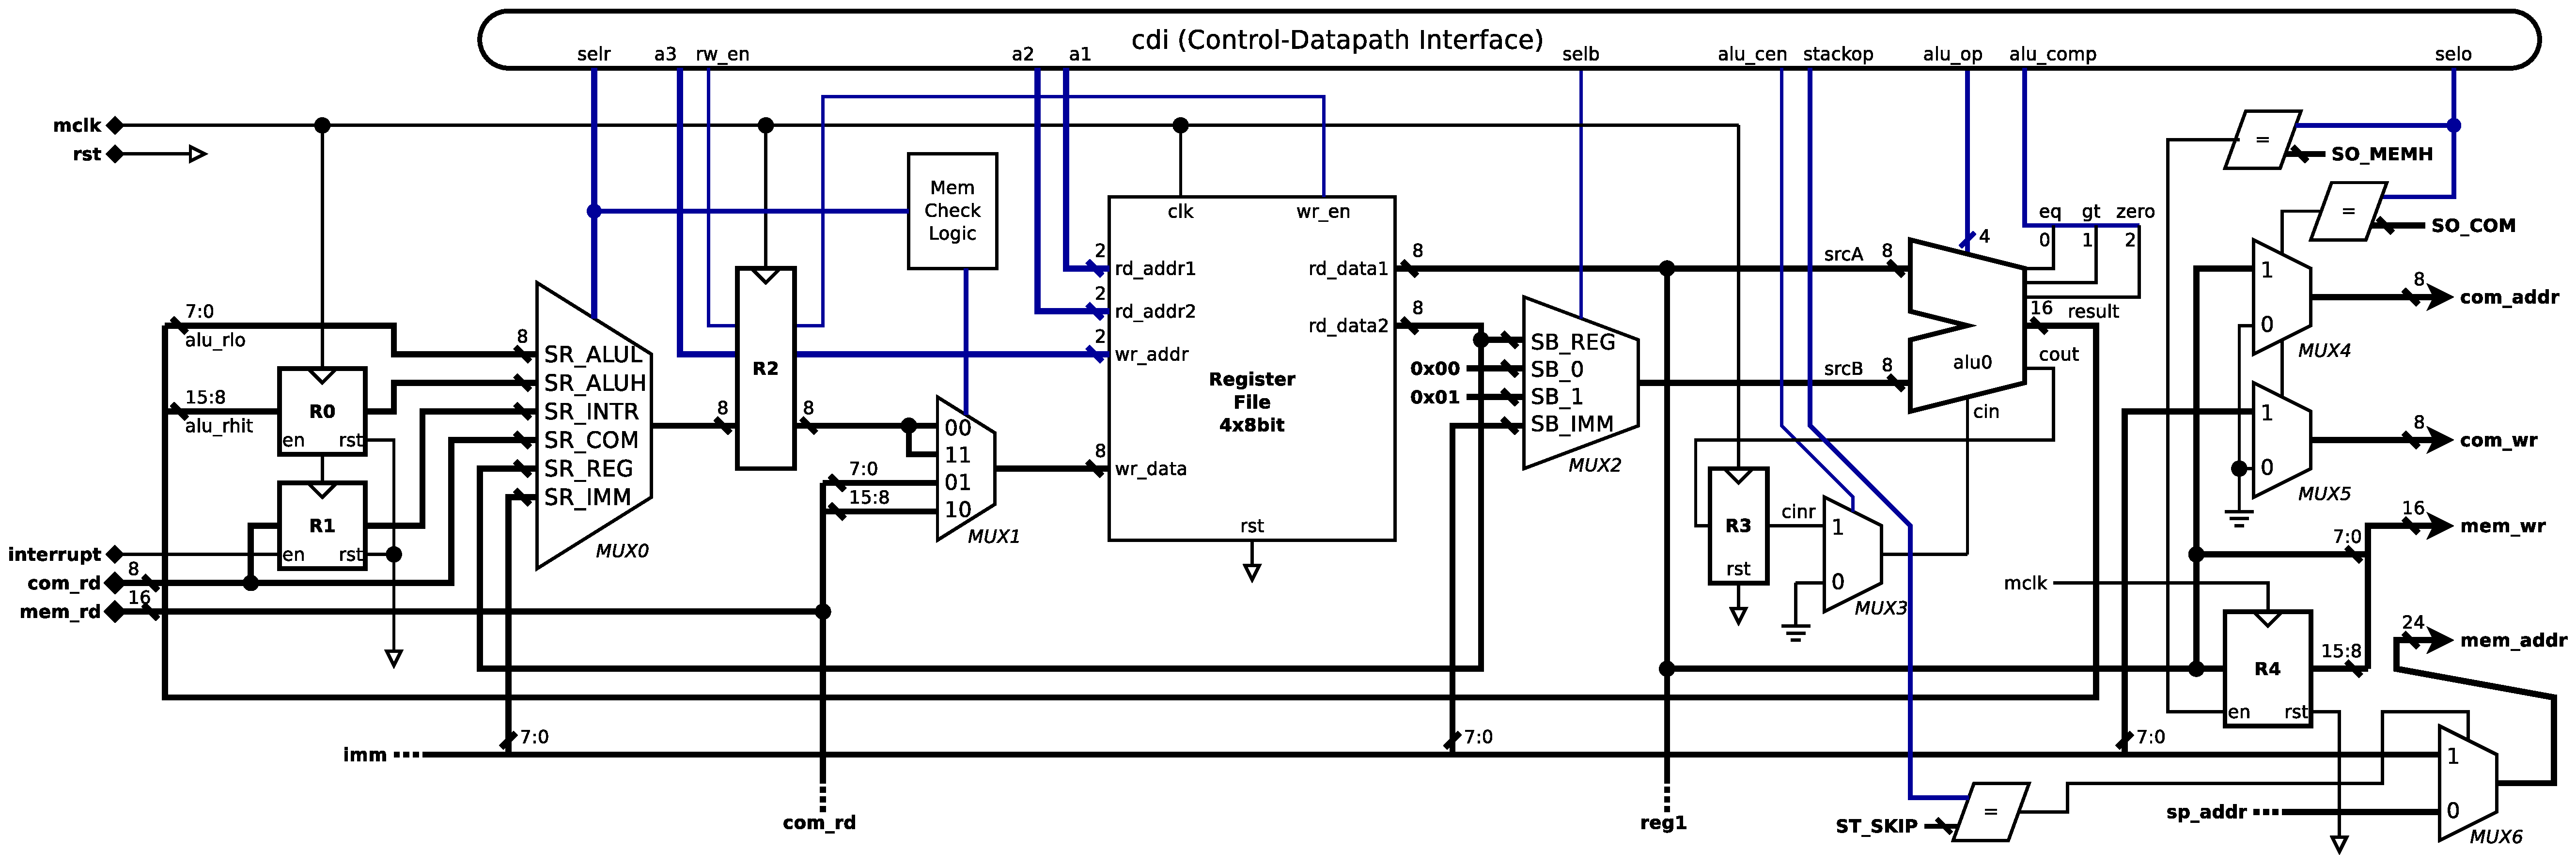
\includegraphics[width=\linewidth]{../resources/datapath.eps}
		\caption{Digital diagram of RISC datapath}
		\label{fig:datapath}	
	\end{figure}
	
	Figure \ref{fig:datapath} above represents a partial RISC datapath. This diagram can be extended to Program counter, Stack pointer and Immediate Override logics are shown in figures \ref{fig:risc_pc}, \ref{fig:risc_stack} and \ref{fig:risc_imo} respectively. CDI (Control-Data Interface) is a HDL (Hardware Description Language) concept that connect datapath and control unit together. The immediate value is provided to datapath by IMO block described in section \ref{subsec:imo}.\\
	Data to register file is selected and saved with \textit{MUX0}. This data is delayed by one cycle with \textit{R2} to match timing that of data taken from the memory. If \texttt{LWLO} or \texttt{LWHI} instructions are executed, \textit{MUX1} select high or low byte from memory to read. In order to compensate for timing, as value written to register file is delayed by one cycle, register file has internal logic that outputs \textit{wr\_data} to \textit{rd\_data1} or/and  \textit{rd\_data2} immediately if \textit{wr\_en} is high and \textit{rd\_addr1} or/and \textit{rd\_addr2} matches \textit{wr\_addr}, making it act more like latch. \\
\end{landscape}
\textit{MUX2}allows to override ALU source B, \textit{R3} and \textit{MUX3} enables control unit to enable ALU carry in bit, allowing multi-word number addition/subtraction. \textit{MUX4} and \textit{MUX5} allows sending data to the COM block with \texttt{COM} instruction. If any other instruction performed, then \textit{0x00} byte for COM address and data is sent, indicating no action. Data can be stored to memory only with a \texttt{SWLO} instruction. It writes high byte value whatever is stored in \textit{R4} register. This buffer can be written to using a \texttt{SWHI} instruction. Therefore, to change only a single byte in a particular memory location, other byte has to be fetched in advanced and used in a \texttt{SWLO} or \texttt{SWHI} instruction. \textit{MUX6} selects memory address value from the \textit{imm} or stack pointer.

\subsubsection{OISC Datapath} \label{subsec:oisc_cells}
OISC datapath only consists of instruction-data bus and a small circuit that connect them to logic blocks that computes the data. These logic blocks can represent ALU operation combinational logic, or any other part of a processor as shown in Figure \ref{fig:oisc_simple}.

Figure \ref{fig:oisc_cell_in} represents a common destination circuit. It checks if a particular logic block destination address matches one in instruction bus, then enables latch and also sets flag that destination is used to the further logic. 
\begin{colfigure}
	\centering
	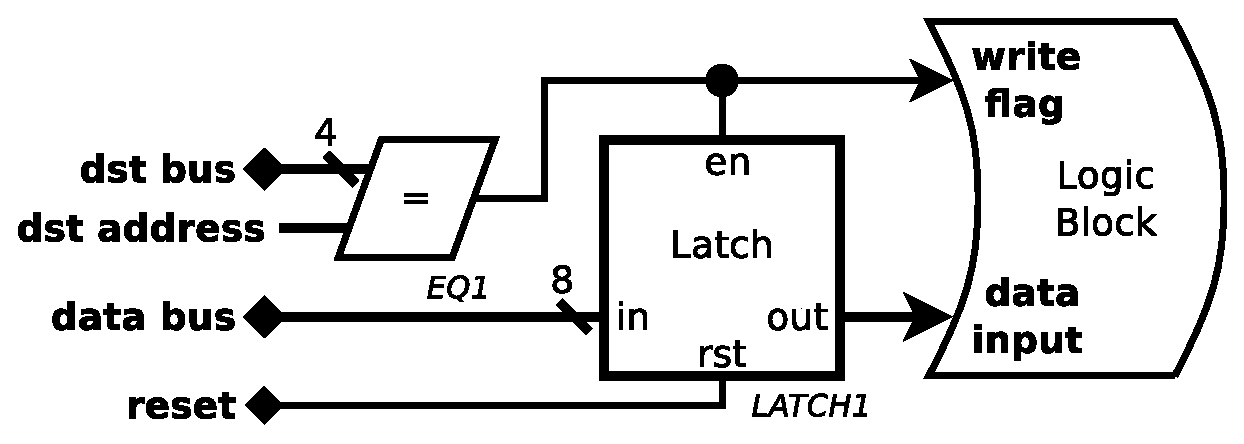
\includegraphics[width=\linewidth]{../resources/oisc_cell_in.eps}
	\captionof{figure}{OISC processor data bus to destination connection logic}
	\label{fig:oisc_cell_in}
\end{colfigure}

Similarly, Figure \ref{fig:oisc_cell_out} represents a source circuit connecting output of a logic block. Logic block can be assumed to only contain combinational logic, therefore a register is placed at the output of it. A buffer \textit{BUF1} is used to connect data in a register \textit{REG1} to the data bus. This ensures that only one bus driver is present, ensuring no data collision. 

\begin{colfigure}
	\centering
	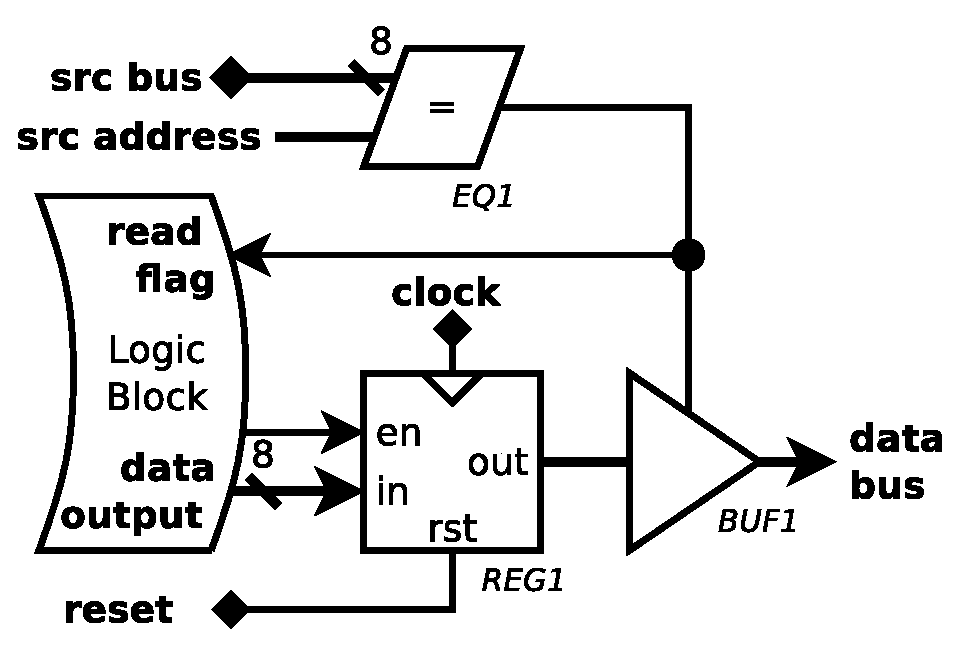
\includegraphics[width=\linewidth]{../resources/oisc_cell_out.eps}
	\captionof{figure}{OISC processor data bus to source connection logic}
	\label{fig:oisc_cell_out}
\end{colfigure}

The general timing is designed so that the information at the source is immediately ready on the data bus at rise of the processor clock. The source is connected to the destination connection where combinational logic is present. 

\subsubsection{OISC Datapath Implementation Problems} \label{subsec:oisc_cell_issue}

The complete implementation using latches for destination logic was not successful. Latches did not operate correctly when synthesised onto FPGA. This issue might be caused by some timing problem between some combination of source and destination logic. The exact cause was not resolved.

As a quick solution, latches at the destination have been replaced with a clocked register that is triggered at negative clock edge, which is opposite to source register trigger. This solution has resolved issue, however it effectively reduces the period of time that data has to propagate though logic blocks between source and destination by two.

\subsection{Stack} \label{subsec:stack}
This section describes dedicated logic for stack pointer control at both processors. The stack pointer starts from the highest memory address value and "stacks" towards lower address values. Both designs were simplified to only operate on two byte addresses, meaning that stack pointer has a constant \texttt{FFh} value at the least significant byte.


\subsubsection{RISC Stack}
The RISC processor implements the stack pointer that is used in \texttt{PUSH}, \texttt{POP}, \texttt{CALL} and \texttt{RET} instructions. Figure \ref{fig:risc_stack} represents the logic diagram for stack pointer. This circuit also supports \textit{pc\_halted} signal from the program counter to prevent the stack pointer from being added by 1 twice during the \texttt{RET} instruction. 

One of the problems with the current stack pointer implementation is 8bit data stored in 16bit memory address, wasting a byte, except when storing the program pointer with \texttt{CALL} instruction. This can be improved by adding a high byte register, however then it would cause complications when a 16bit program pointer is stored with \texttt{CALL} instruction. This can still be improved with a more complex circuit, or by using memory cache with 8bit data input. However, with the current implementation this does not affect processor comparison, it only increases stack size in memory.

\begin{figure*}
	\centering
	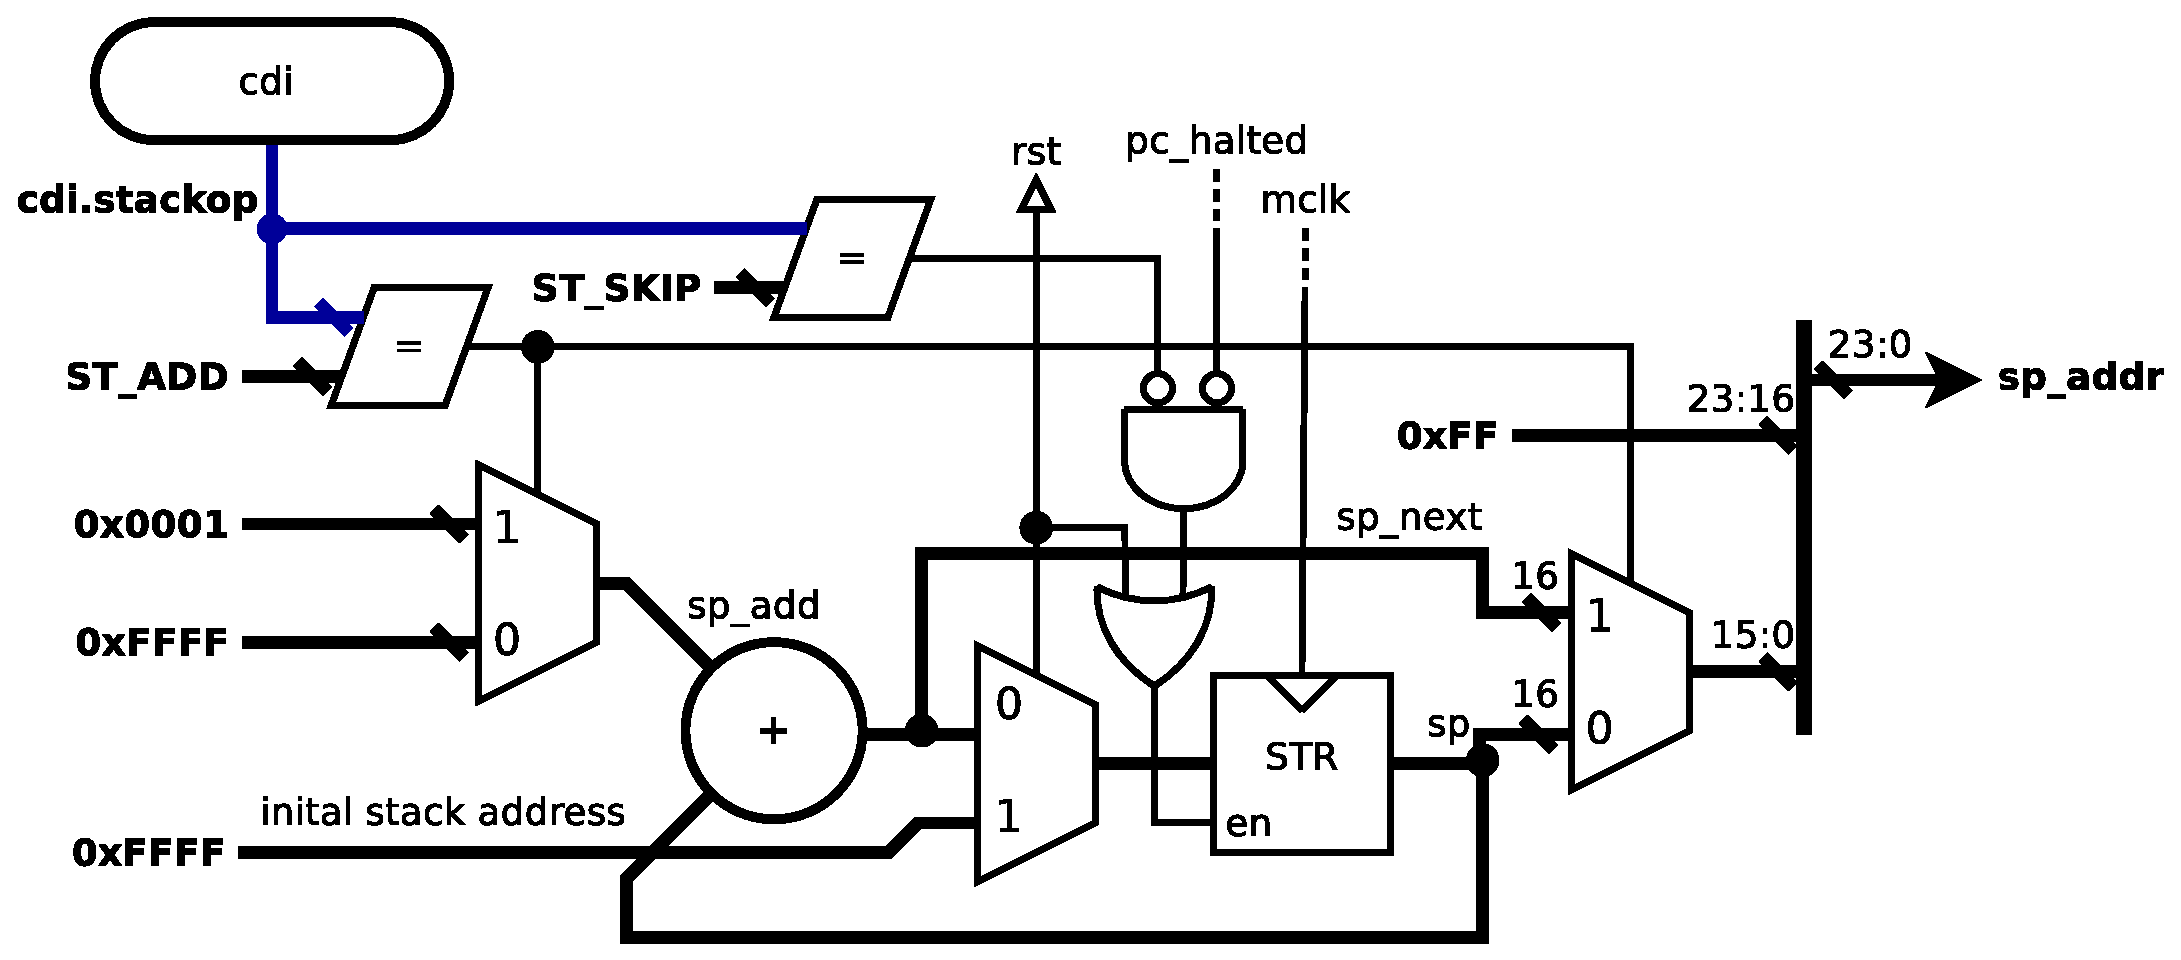
\includegraphics[scale=0.4]{../resources/risc_stack.eps}
	\caption{Digital diagram of RISC stack pointer logic}
	\label{fig:risc_stack}
\end{figure*}

\subsubsection{OISC Stack}

The stack pointer circuit in OISC is very similar to RISC. When reset, push or pop flags are set, it changes the state of stack pointer by adding or subtracting its value by one, or resetting it to default. Logic diagram is shown in Figure \ref{fig:oisc_stack}.
\begin{figure*}[b]
	\centering
	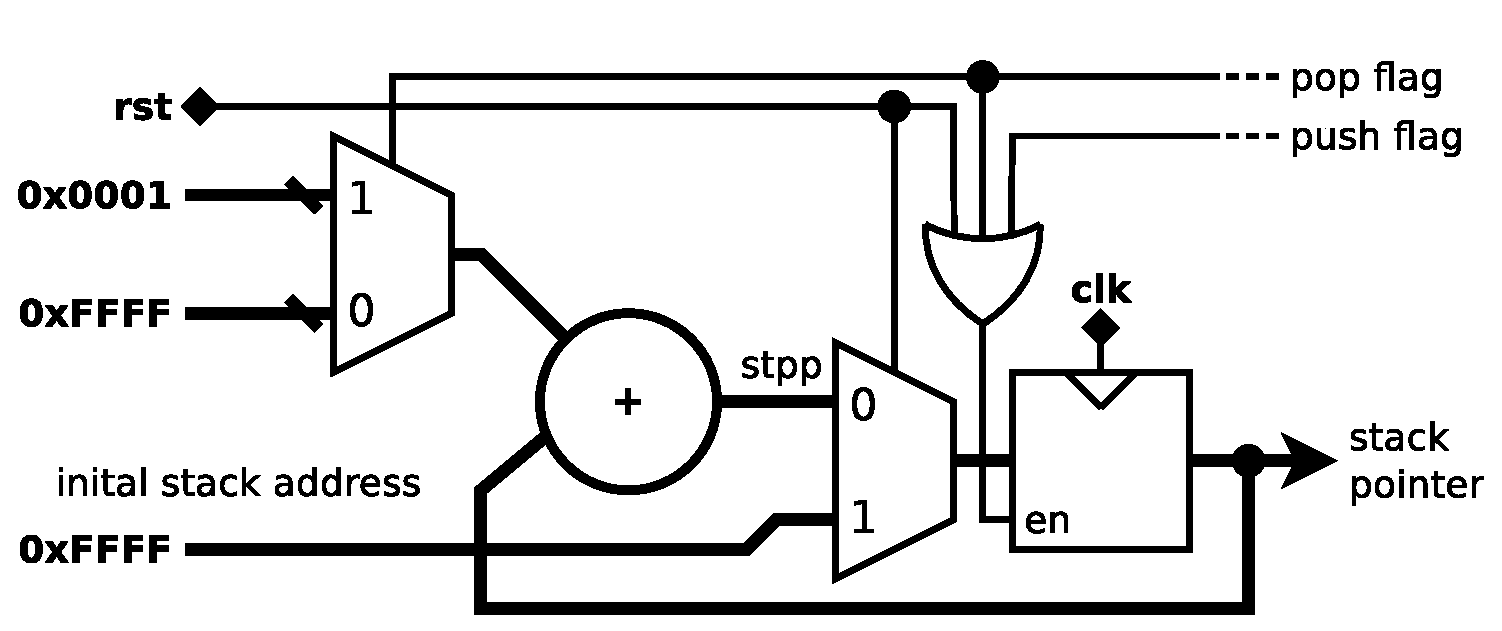
\includegraphics[scale=0.4]{../resources/oisc_stack.eps}
	\caption{Digital diagram of OISC stack pointer logic}
	\label{fig:oisc_stack}
\end{figure*}

Logic diagram of stack control unique to OISC processor is shown in Figure \ref{fig:oisc_stack_2}. Push and pop flags are taken from the source and destination logic. A cached value of last stored value is kept, so that it would be immediately available on source request. Pop flag is delayed by one clock cycle. This ensures that once stack value is popped, lower stack value is written into the cache during next the clock cycle. Note that there is an issue with this design, stack source or destination instruction cannot be used together with other stack or memory operations as it creates a collision accessing system memory at the same time. This collision can be avoided with software however. 
\begin{figure*}
	\centering
	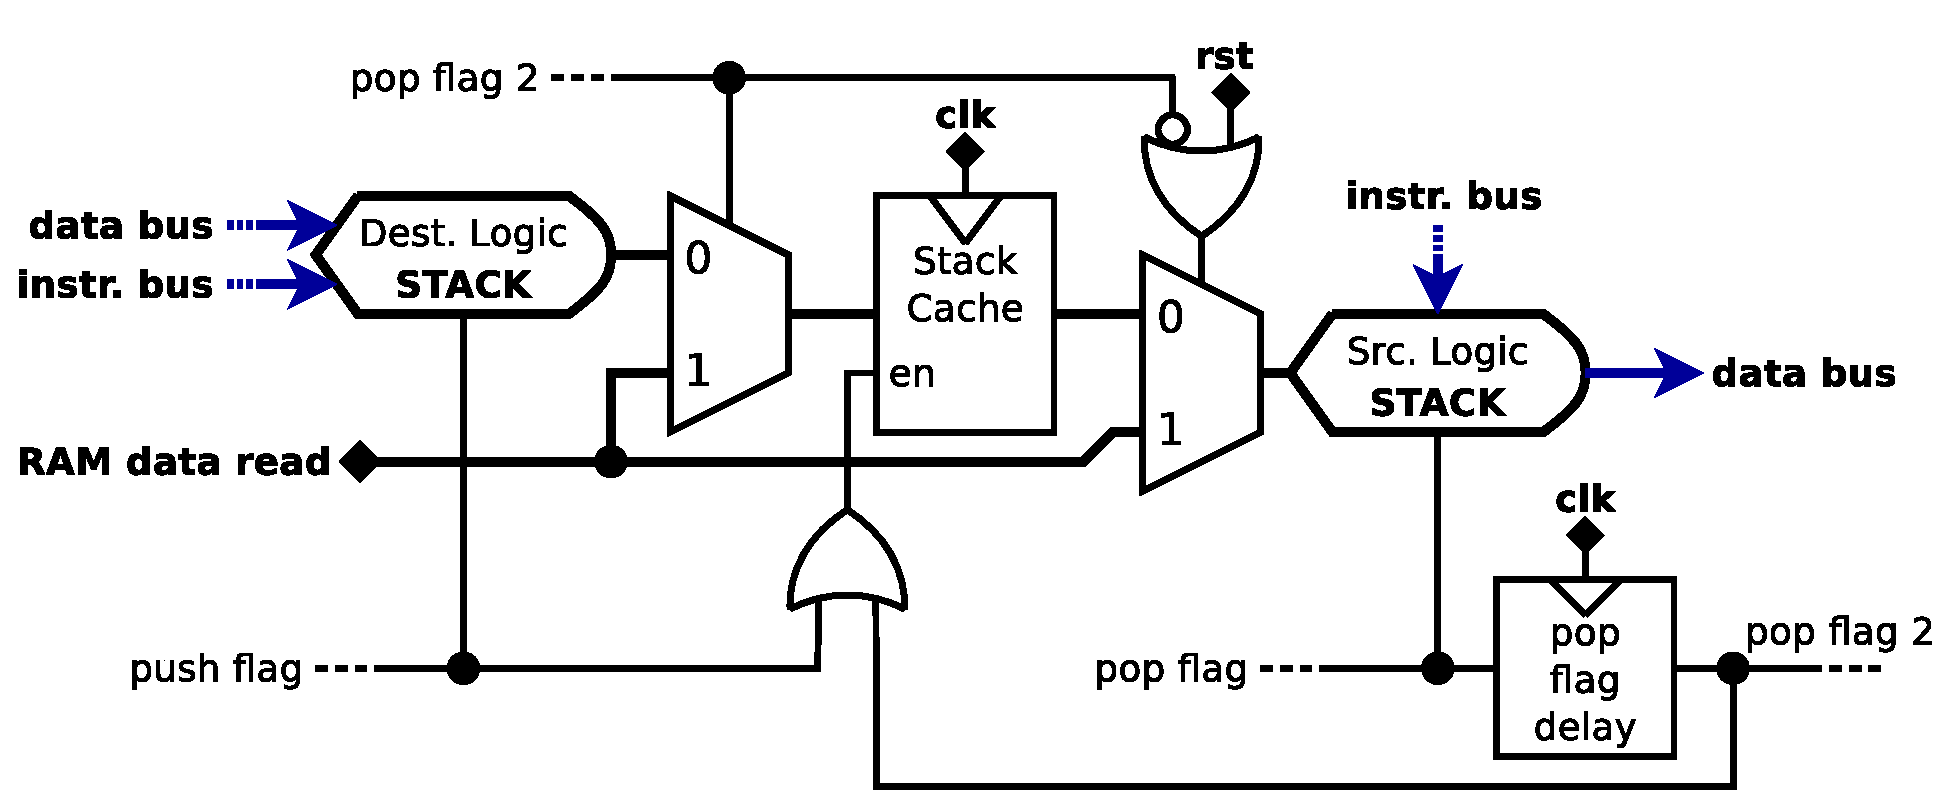
\includegraphics[scale=0.4]{../resources/oisc_stack_2.eps}
	\caption{Digital diagram of OISC stack control logic}
	\label{fig:oisc_stack_2}
\end{figure*}

\subsection{Program Counters} \label{subsec:pc}
In this subsection, program counter and their differences will be described.

\subsubsection{RISC Program Counter}

\begin{figure*}[h!]
	\centering
	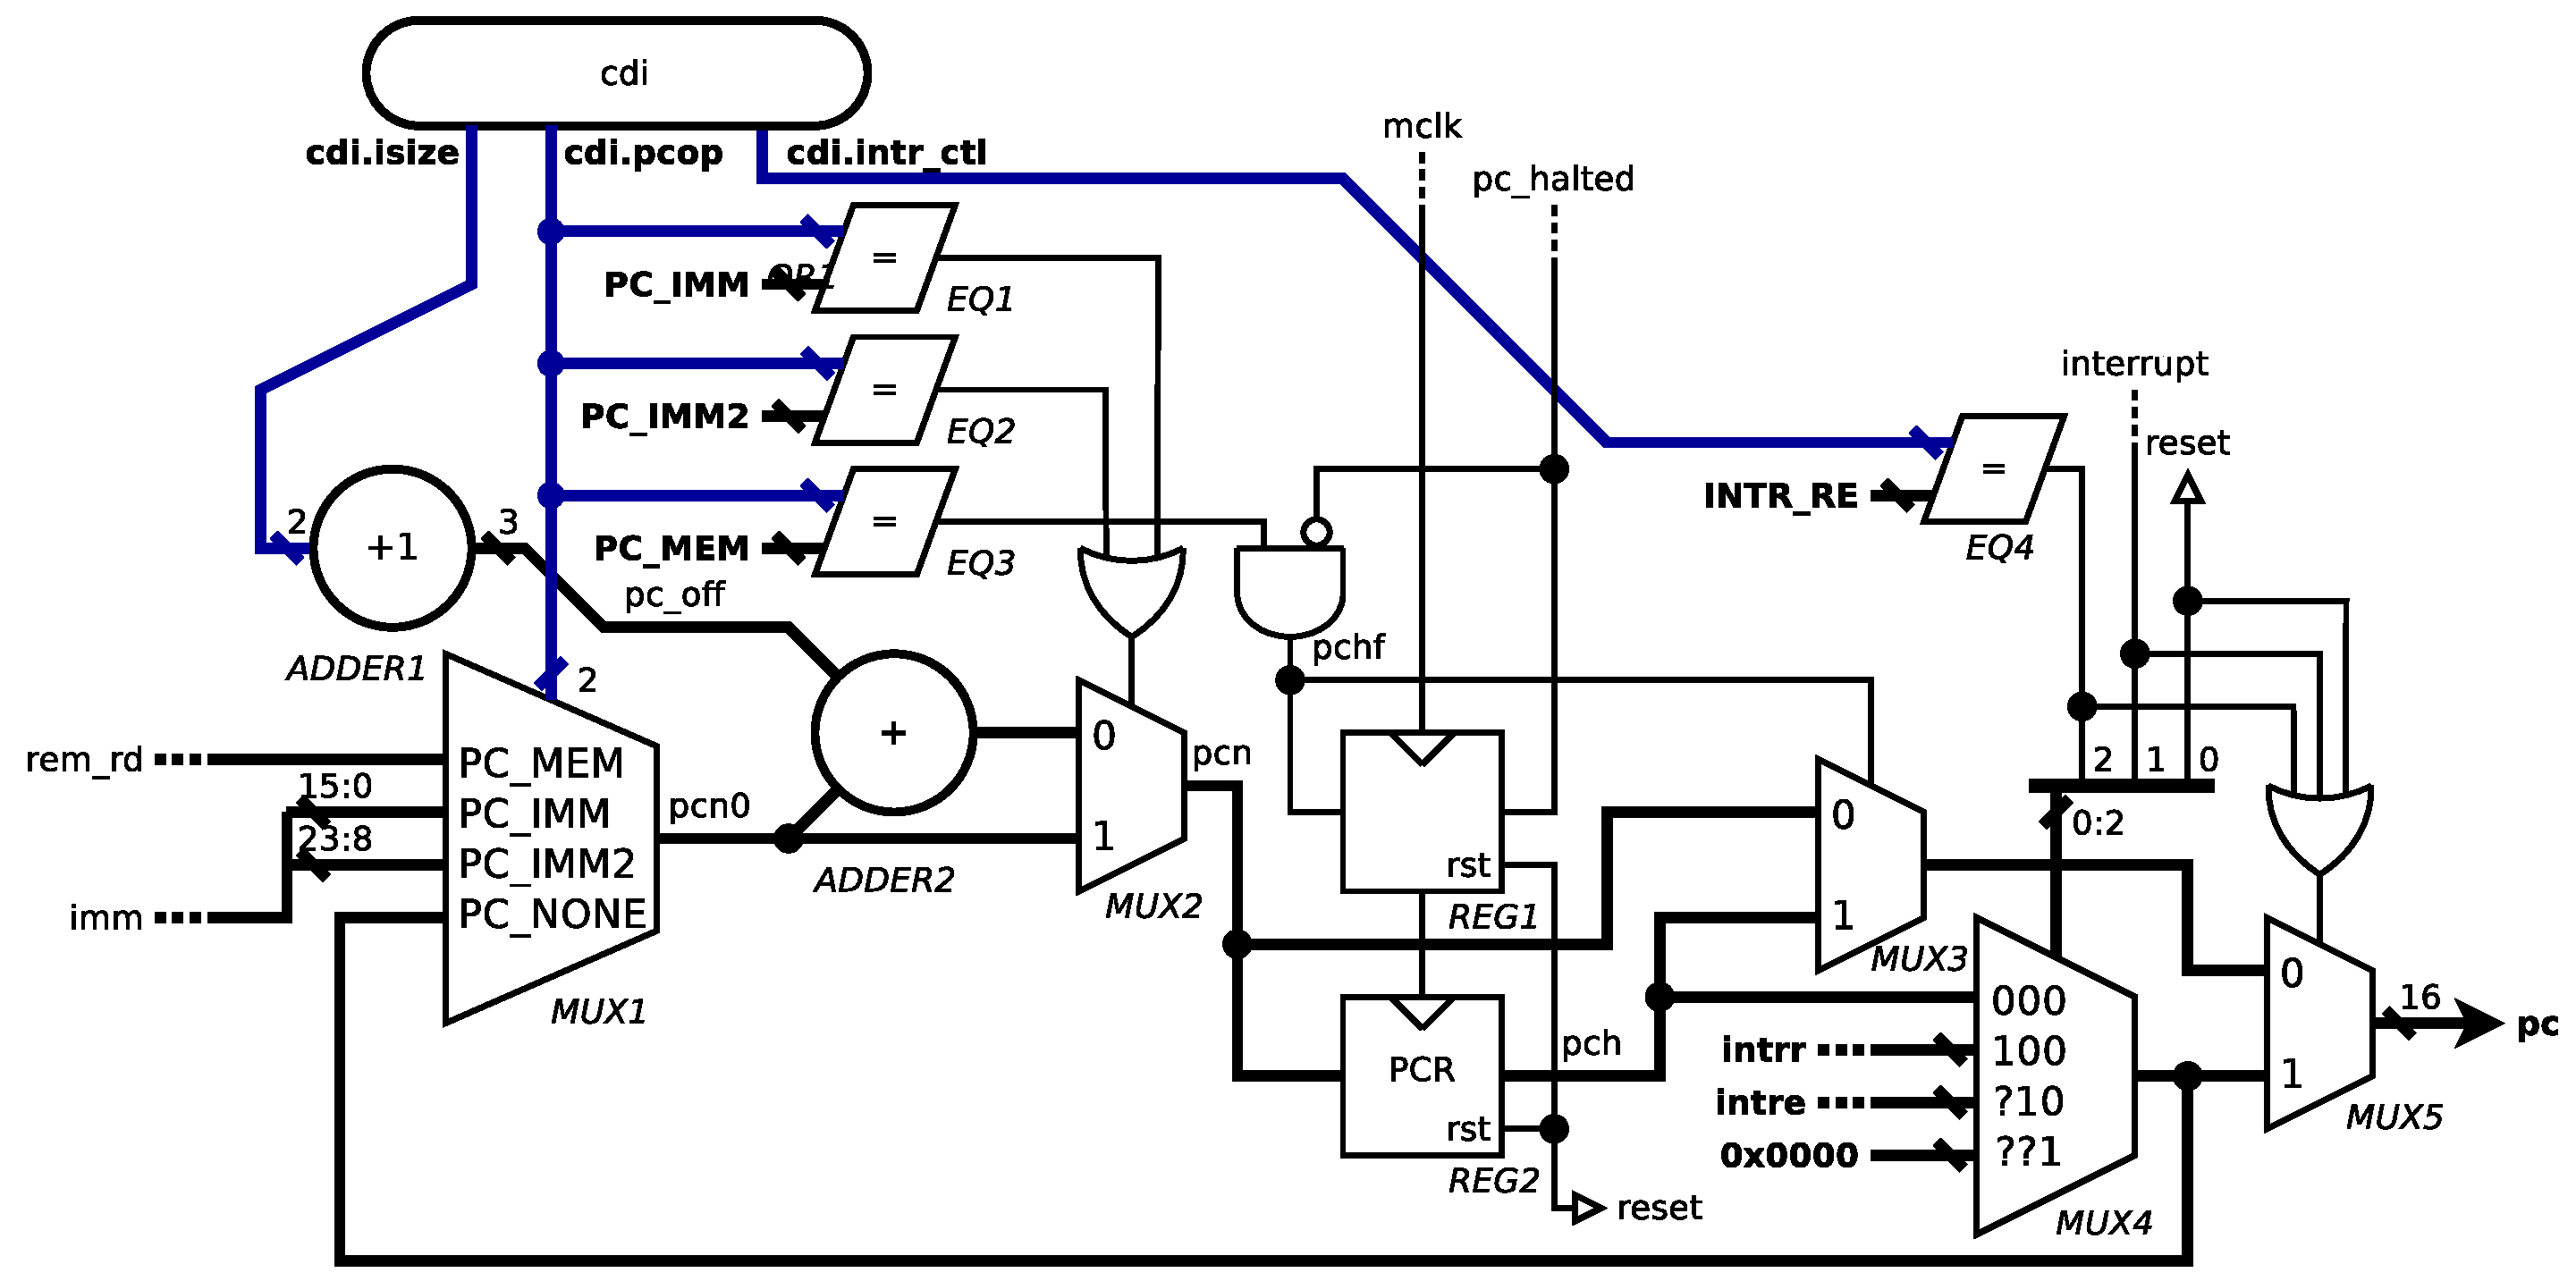
\includegraphics[width=\linewidth]{../resources/risc_pc.eps}
	\caption{Digital diagram of RISC program counter}
	\label{fig:risc_pc}
\end{figure*}

Figure \ref{fig:risc_pc} represents the digital diagram for a program counter. There are a few key features about this design: it can take values from memory for \texttt{RET} instruction; immediate value (\textit{PC\_IMM2} is shifted by one byte to allow \texttt{BEQ}, \texttt{BGT}, \texttt{BGE} instructions as first immediate byte used as ALU source B); it can jump to an interrupt address; it produces a \textit{pc\_halted} signal when memory is read (\texttt{RET} instruction takes two cycles, because cycle one fetches the address from stack and second cycle fetches the instruction from the instruction memory).

\subsubsection{OISC Program Counter}\label{subsec:oisc_pc}
 
OISC program counter is much simpler than RISC, as it does not have variable length instruction, delay flags for \texttt{RET} operation, or logic for selecting branch source address. 
 
\begin{colfigure}
	\centering
	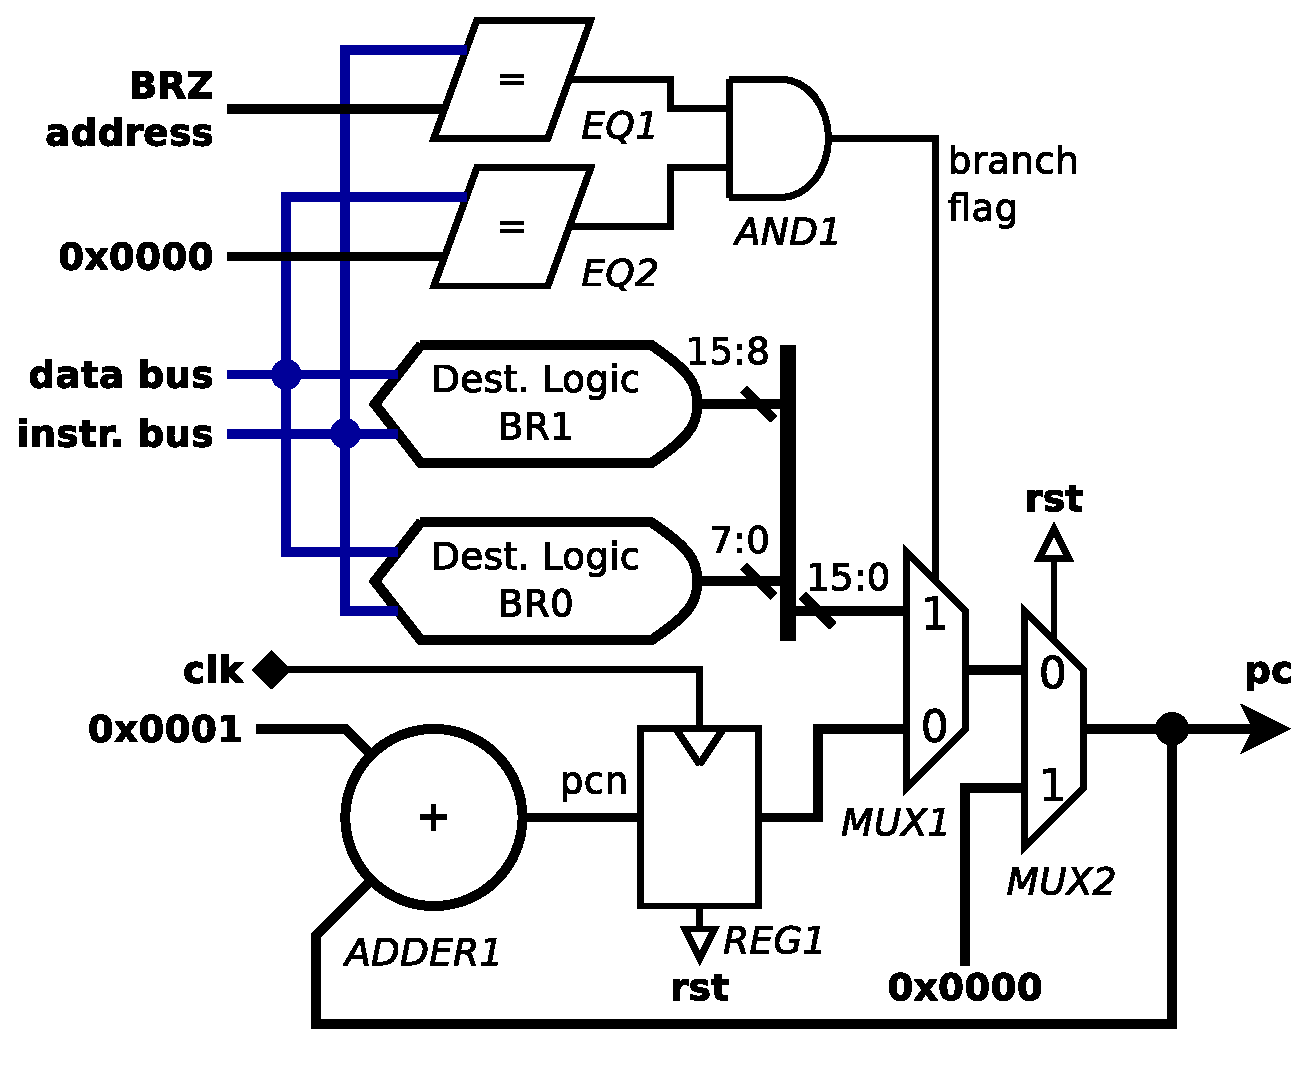
\includegraphics[width=\linewidth]{../resources/oisc_pc.eps}
	\captionof{figure}{Digital diagram of OISC program counter}
	\label{fig:oisc_pc}
\end{colfigure}

Looking at Figure \ref{fig:oisc_pc} bottom, the basic operation is to just add one to previous program counter with \textit{ADDER1} and \textit{REG1}, reset it to zero at reset with \textit{MUX2}. Two destination logic blocks are used as accumulators to store branch address. Once an instruction with the \texttt{BRZ} destination is executed, comparator \textit{EQ2} checks if the data bus value is equal to zero. If this condition is met, it enables \textit{MUX1} and overrides program counter to address stored in \texttt{BR0} and \texttt{BR1} accumulators. Unlike in RISC however, it requires three instructions to set new address and jump. Similarly, \textit{CALL} and \textit{RET} requires five and three instructions respectively. RISC equivalent instructions are show in Listing \ref{code:oisc_jump}.

\begin{blockpage}
	\begin{lstlisting}[frame=single, emph={JUMP, CALL, RET, return}, label=code:oisc_jump, caption={OISC assembly code emulating RISC \texttt{JUMP}, \texttt{CALL} and \texttt{RET} instructions.}]
%macro JUMP 1
  BR1 %1 @1
  BR0 %1 @0
  BRZ 0x00
%endmacro

%macro CALL 1
  BR1 %1 @1
  BR0 %1 @0
  STACK %%return @1
  STACK %%return @0
  BRZ 0x00
  %%return:
%endmacro

%macro RET 0
  BR0 STACK
  BR1 STACK
  BRZ 0x00
%endmacro
	\end{lstlisting}
\end{blockpage}

\subsection{Arithmetic Logic Unit}\label{subsec:alu}

\begin{figure*}[b]
\centering
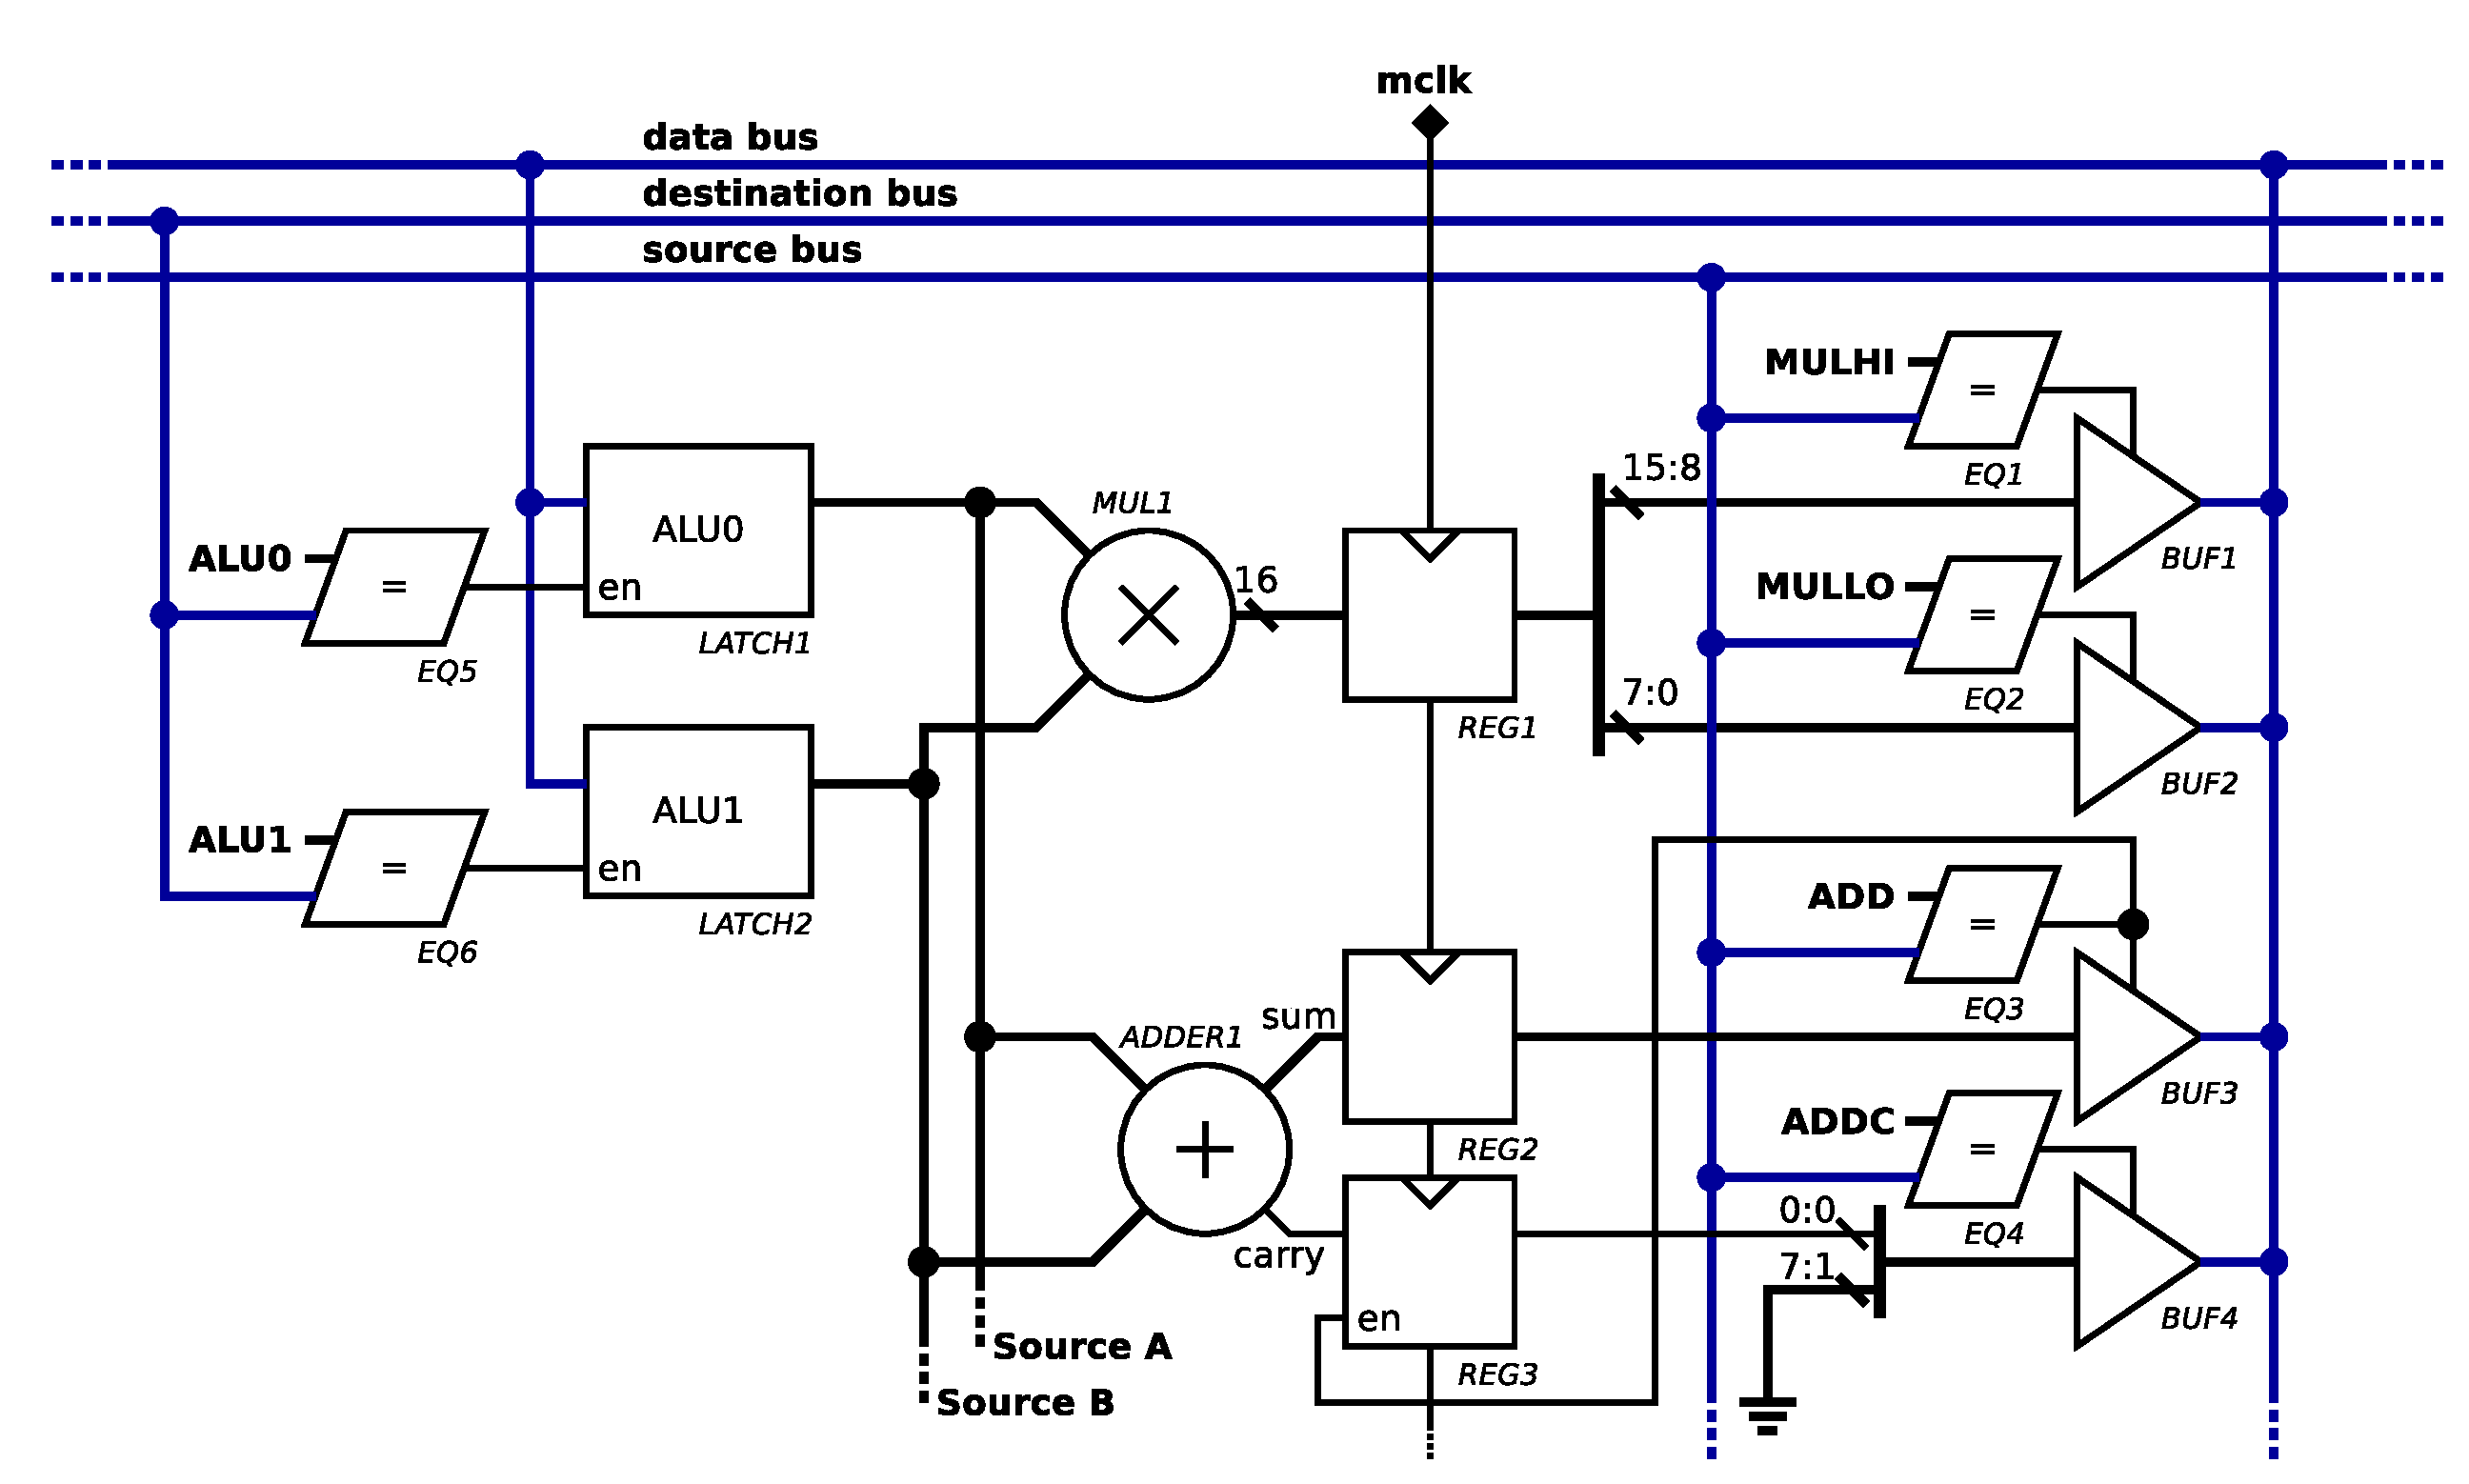
\includegraphics[scale=0.35]{../resources/oisc_alu.eps}
\caption{Digital diagram of OISC partial ALU logic}
\label{fig:oisc_alu}
\end{figure*}

This section will discuss ALU implementations of both processors. For fair comparison between OISC and RISC, ALU in both system will have the same capabilities as described in Table \ref{tab:alu_set}.

\begin{blockpage}
	\arrayrulecolor{black}
	\begin{tabular}{| c | p{0.75\linewidth} |} \hline 
		\rowcolor[rgb]{0.82,0.82,0.82}
		Name & Description \\\hline
		\arrayrulecolor[rgb]{0.82,0.82,0.82}
		ADD & Arithmetic addition (inc. carry) \\\hline
		SUB & Arithmetic subtraction (inc. carry) \\\hline
		AND & Bitwise AND \\\hline
		OR  & Bitwise OR \\\hline
		XOR & Bitwise XOR \\\hline
		SLL & Shift left logical \\\hline
		SRL & Shift right logical \\\hline
		ROL & Shifted carry from previous SLL \\\hline
		ROR & Shifted carry from previous SRL \\\hline
		MUL & Arithmetic multiplication \\\hline
		DIV & Arithmetic division \\\hline
		MOD & Arithmetic modulo \\
		\arrayrulecolor[rgb]{0,0,0}\hline
	\end{tabular}
	\captionof{table}{\textit{Supported ALU commands for both processors}}
	\label{tab:alu_set}
\end{blockpage}

\subsubsection{OISC ALU}
Due to the structure of the OISC processor, ALU source A and B are two latches that are written into when \texttt{ALU0} or \texttt{ALU1} destination address is present. ALU sources are connected with every ALU operator and performed in single clock cycle. This value is stored in a register so that it would be immediately available in a next clock cycle as a source data, as explained in \nameref{subsec:oisc_cells} Section. Figure \ref{fig:oisc_alu} represents a logic diagram of ALU with only an addition and multiplication operations present. Note that the output of \textit{EQ3} is connected to enable of \textit{REG3}, enabling output of carry to be only read after \texttt{ADD} source is requested. Similar configuration is also used for \texttt{SUB}, \texttt{ROL} and \texttt{ROR} operations.

\subsubsection{RISC ALU}
The RISC processor has very similar structure to OISC, however with two exceptions. Inputs to ALU comes from datapath data router logic. Output buffers are replaced by one multiplexer that selects a single output from all ALU operations. Another point is that RISC ALU output is 16bit, higher byte saved in "ALU high byte register" for \texttt{MUL}, \texttt{MOD}, \texttt{ROL} and \texttt{ROR} operations. This register is accessible with \texttt{GETAH} instruction.

\subsection{Program Memory}\label{subsec:memory}
This section describes how instruction memory (ROM) is implemented for both processors.

\begin{figure*}[b]
	\centering
	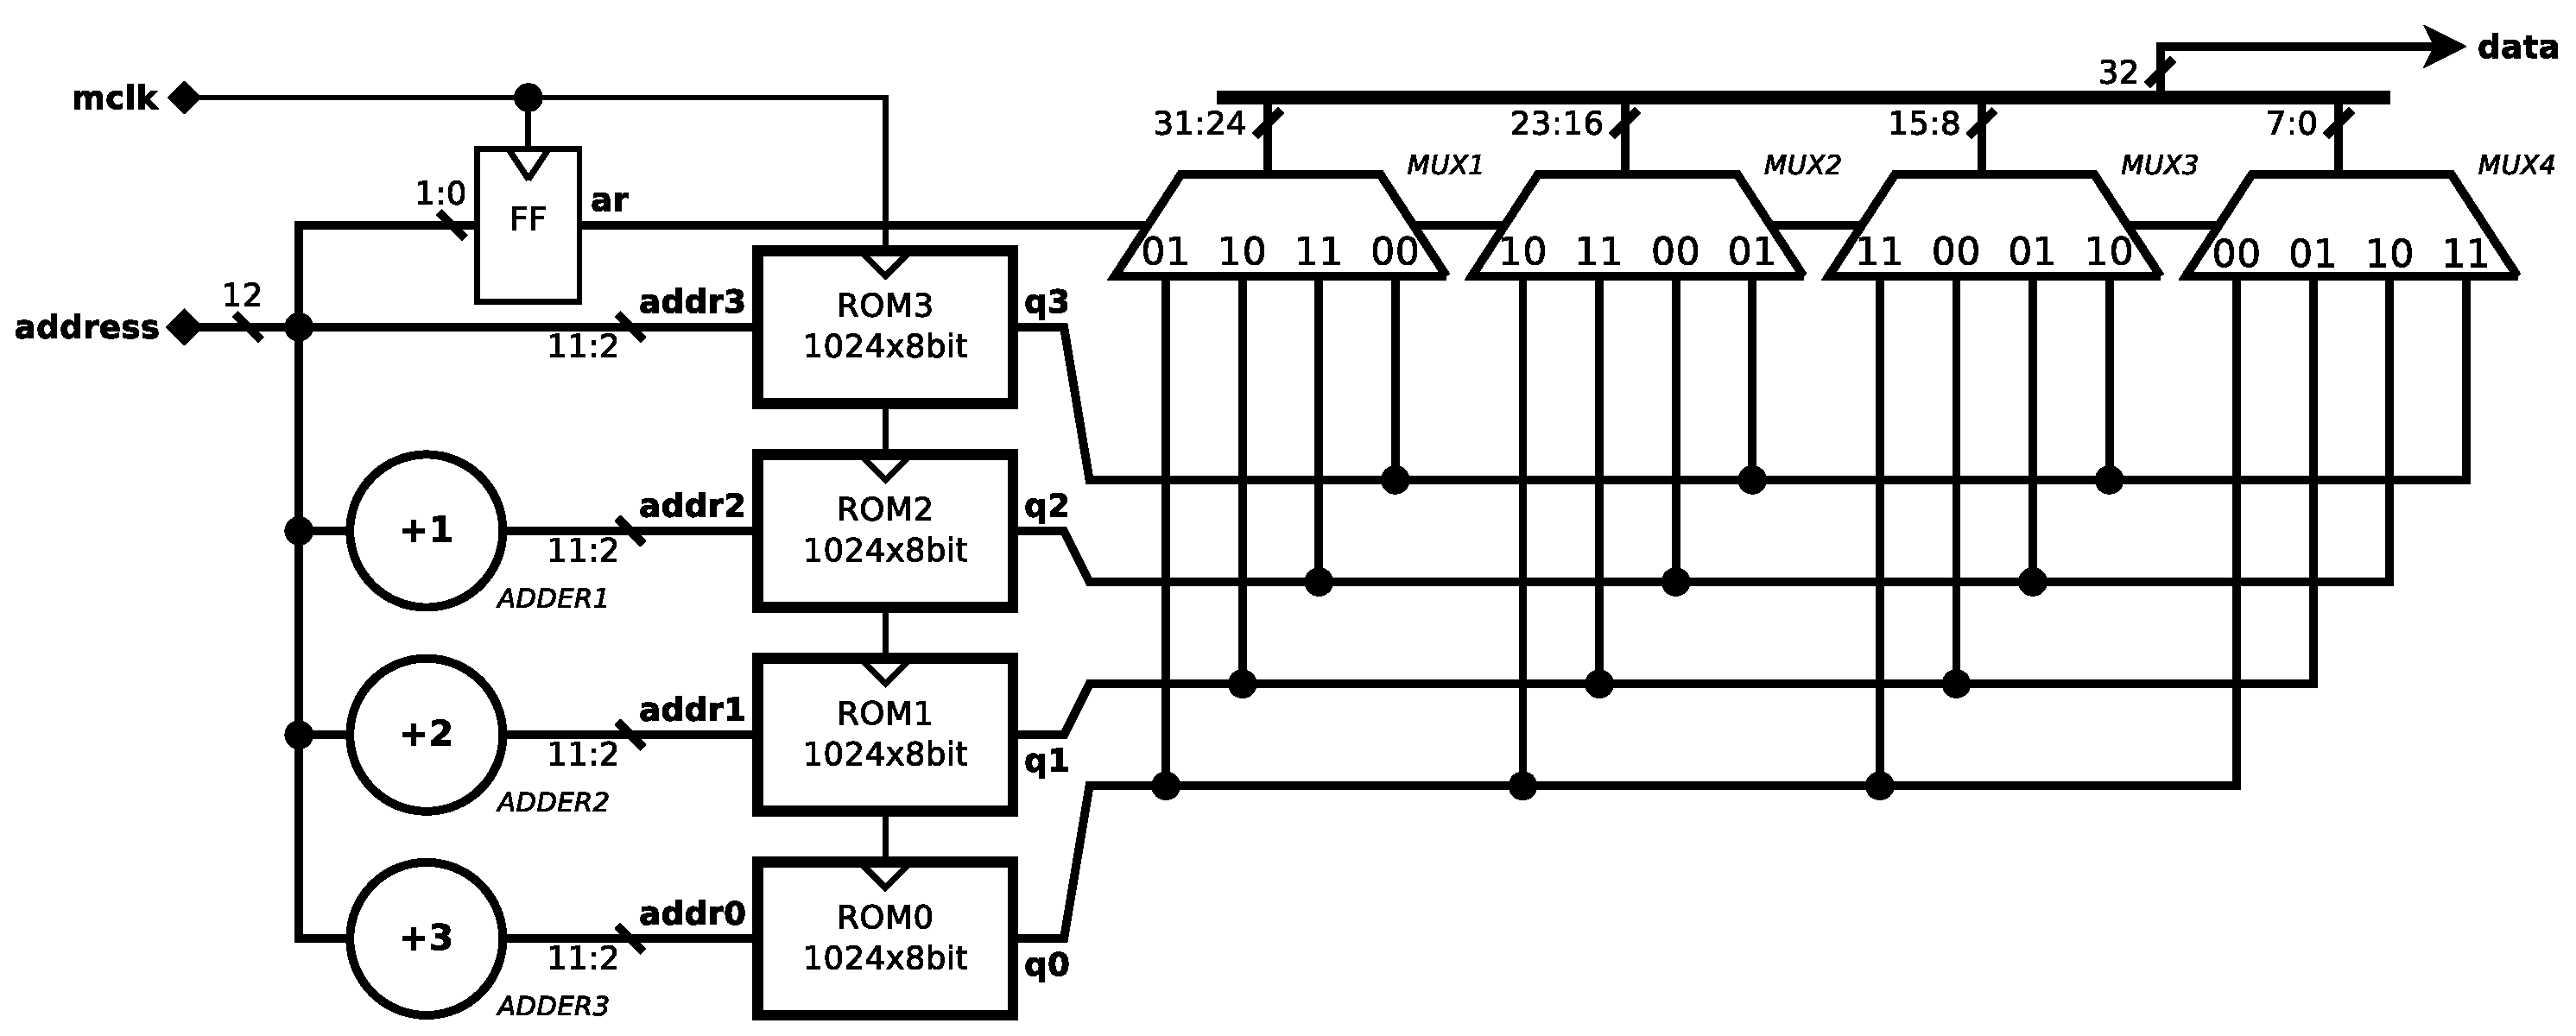
\includegraphics[width=\linewidth]{../resources/risc_mem.eps}
	\caption{Digital diagram of RISC sliced ROM memory logic}
	\label{fig:risc_mem}
\end{figure*}

\subsubsection{RISC Program Memory}
In order to allow a dynamic instruction size from one to four bytes, a special memory arrangement is made. A system was re-
quired to access a word (8bits) from memory and next three words, meaning that memory cannot simply be packed to four word segments. To achieve desired functionality, four ROM blocks been utilised, each containing one fourth of sliced original data. Input address is offset by adders \textit{ADDER1-3} and further divided by value four, which is done by removing two least significant bits at \textbf{addr0-3}. 
Before concatenating output of each ROM block into final four bytes, ROM outputs \textbf{q0-3} are rearranged depending on \textbf{ar} signal. Note that \textit{MUX1-4} each input is different, this may be better visualised with Verilog code in listing \ref{code:rom_switch}.


\begin{blockpage}
\begin{lstlisting}[frame=single, language=Verilog, caption={RISC sliced ROM memory multiplexer arrangement Verilog code}, emph={ar, data}, label=code:rom_switch]
case(ar)
  2'b00: data={q3,q2,q1,q0};
  2'b01: data={q0,q3,q2,q1};
  2'b10: data={q1,q0,q3,q2};
  2'b11: data={q2,q1,q0,q3};
endcase
\end{lstlisting}
\end{blockpage}

\subsubsection{OISC Program Memory}\label{subsec:oisc_mem}
OISC instructions are fixed 13 bits, this non-standard memory word size causes some difficulties. To implement ROM in FPGA, Altera Cyclone IV M9K configurable memory blocks were used. Each blocks has 9kB of memory, each set as 1024x9bit configuration. Combining three these blocks together yields 27bits if readable data in single clock cycle. To store instruction code to such configuration, pairs of instruction machine code sliced into three parts plus one bit for parity check, see figure \ref{fig:oisc_memory_slice}. Circuit extracting each instruction is fairly simple, shown in figure \ref{fig:oisc_mem}.

\begin{figure*}[t]
\begin{gather*}
\overunderbraces{&\br{1}{ROM0}&\br{2}{ROM1}&\br{2}{ROM2}}%
{&
\colorbox{c1}{\scalebox{0.75}{00}}\,
\colorbox{c1}{\scalebox{0.75}{01}}\,
\colorbox{c1}{\scalebox{0.75}{02}}\,
\colorbox{c1}{\scalebox{0.75}{03}}\,
\colorbox{c1}{\scalebox{0.75}{04}}\,
\colorbox{c1}{\scalebox{0.75}{05}}\,
\colorbox{c1}{\scalebox{0.75}{06}}\,
\colorbox{c1}{\scalebox{0.75}{07}}\,
\colorbox{c1}{\scalebox{0.75}{08}}\,&
\colorbox{c1}{\scalebox{0.75}{09}}\,
\colorbox{c1}{\scalebox{0.75}{10}}\,
\colorbox{c1}{\scalebox{0.75}{11}}\,
\colorbox{c1}{\scalebox{0.75}{12}}\,&
\colorbox{c2}{\scalebox{0.75}{13}}\,
\colorbox{c2}{\scalebox{0.75}{14}}\,
\colorbox{c2}{\scalebox{0.75}{15}}\,
\colorbox{c2}{\scalebox{0.75}{16}}\,
\colorbox{c2}{\scalebox{0.75}{17}}\,&
\colorbox{c2}{\scalebox{0.75}{18}}\,
\colorbox{c2}{\scalebox{0.75}{19}}\,
\colorbox{c2}{\scalebox{0.75}{20}}\,
\colorbox{c2}{\scalebox{0.75}{21}}\,
\colorbox{c2}{\scalebox{0.75}{22}}\,
\colorbox{c2}{\scalebox{0.75}{23}}\,
\colorbox{c2}{\scalebox{0.75}{24}}\,
\colorbox{c2}{\scalebox{0.75}{25}}\,&
\colorbox{c3}{\scalebox{0.75}{26}}\,&
}%
{&\br{2}{InstrA}&\br{2}{InstrB}&\br{1}{parity}}
\end{gather*}
\caption{OISC three memory words composition. Number inside box represents bit index.}
\label{fig:oisc_memory_slice}
\end{figure*}

\begin{figure*}[t]
	\centering
	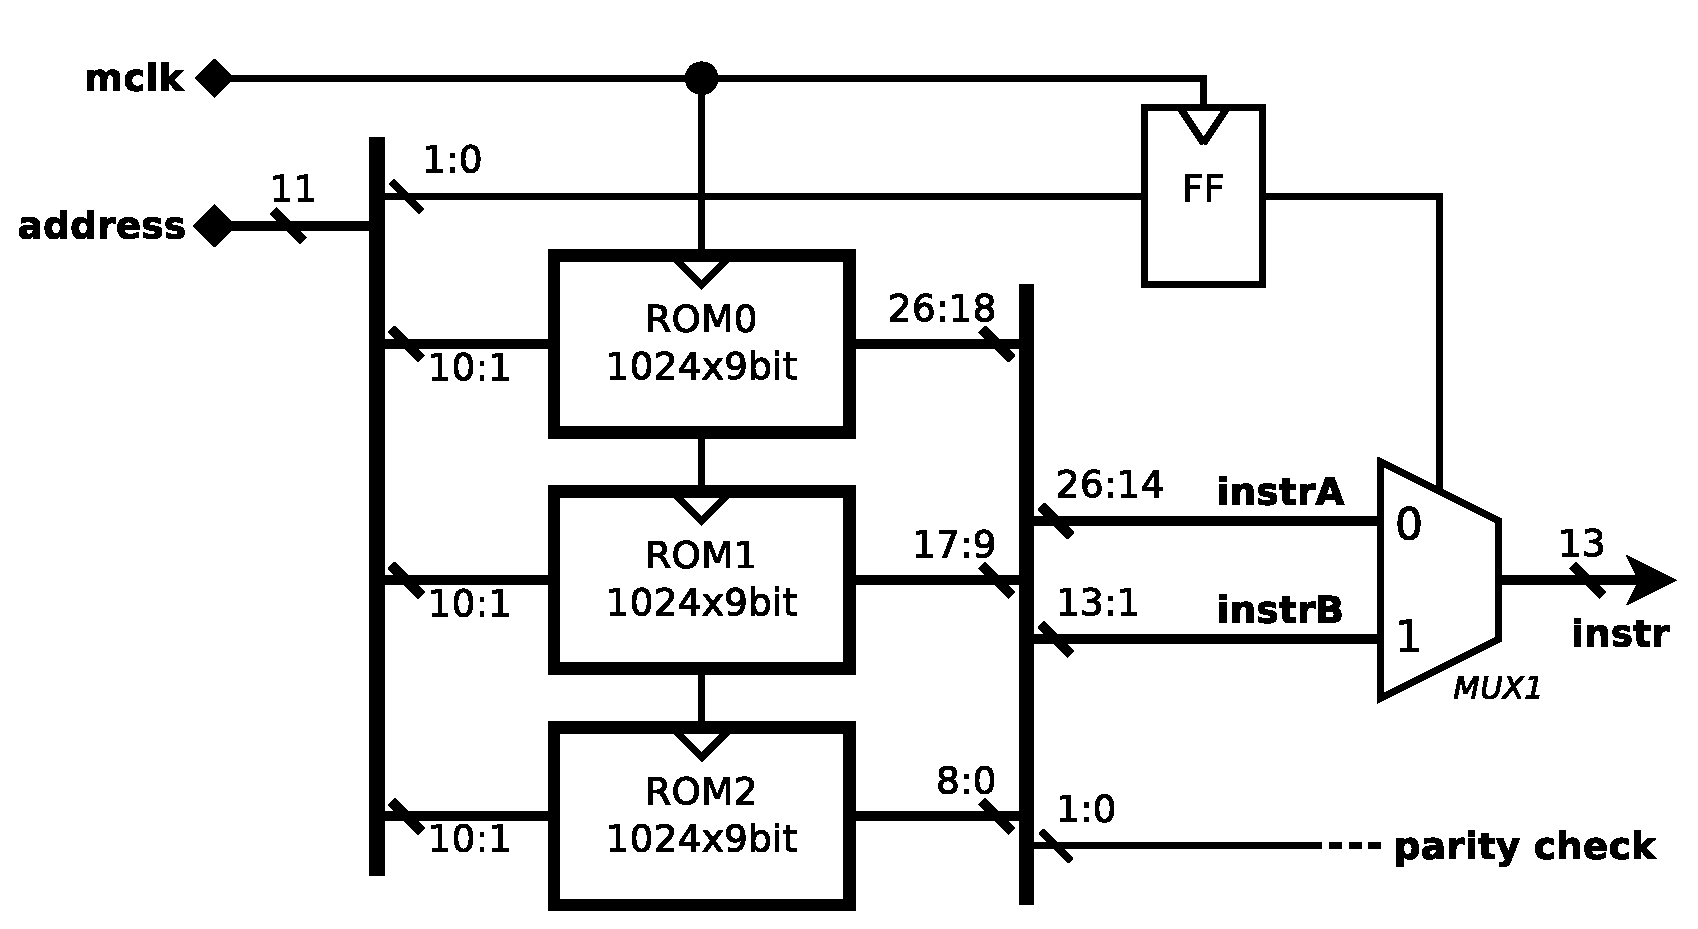
\includegraphics[scale=0.4]{../resources/oisc_mem.eps}
	\caption{Digital diagram of OISC instruction ROM logic}
	\label{fig:oisc_mem}
\end{figure*}

\subsection{Instruction decoding}\label{subsec:imm_values}
This section describes RISC and OISC differences between instruction decoding and immediate value handling.
\subsubsection{RISC IMO} \label{subsec:imo}
Already described in previous section \ref{subsec:memory}, instruction from the memory comes as four bytes. The least significant byte is sent to control block, other three bytes are sent to the immediate override block (IMO) shown in figure \ref{fig:risc_imo}. These three bytes are labelled as \textbf{immr}. 

\begin{figure*}
	\centering
	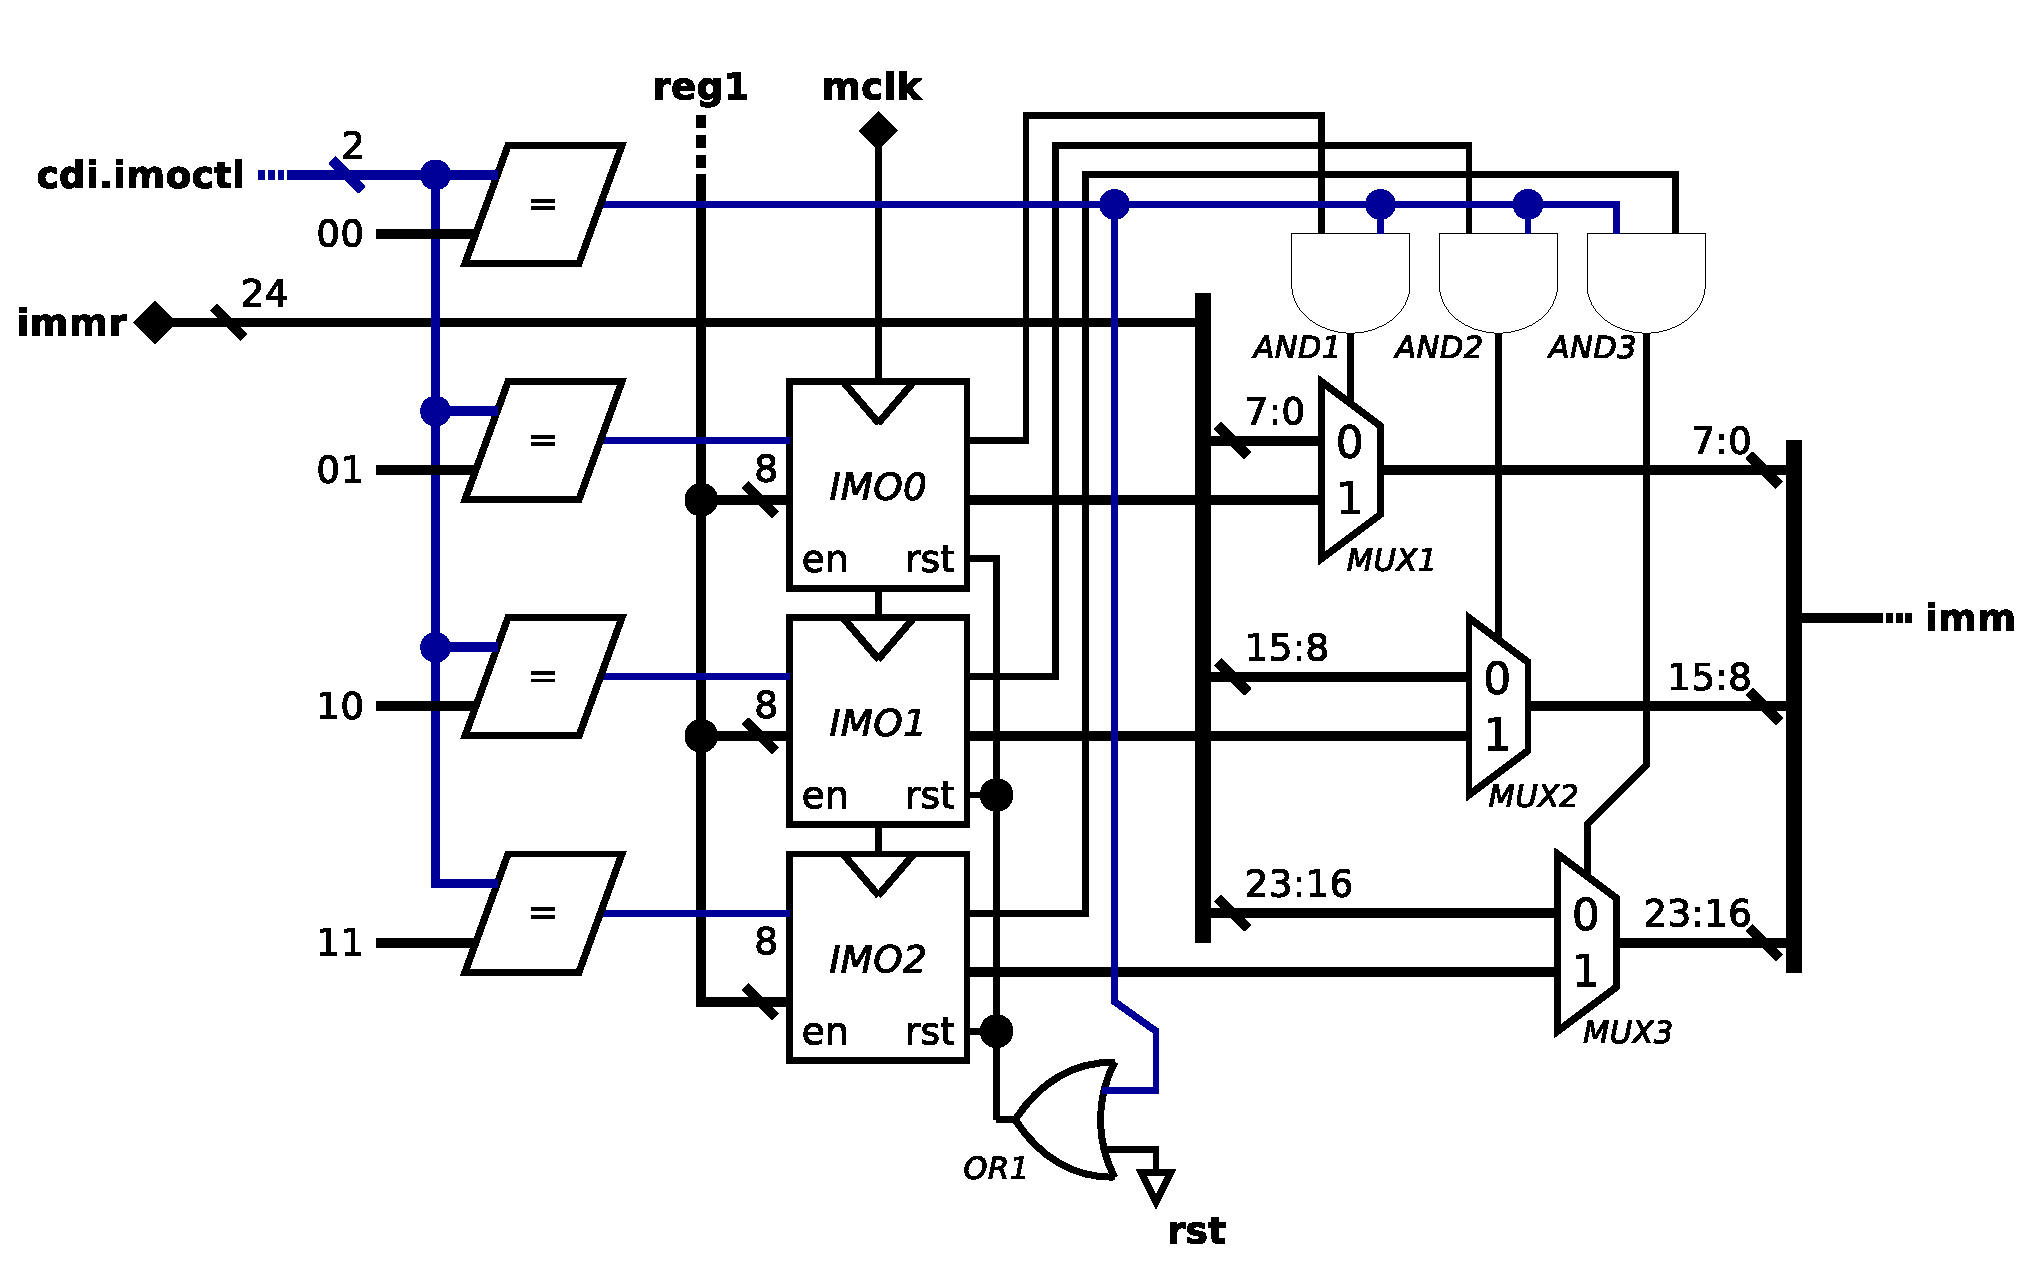
\includegraphics[scale=0.4]{../resources/risc_imo.eps}
	\caption{Digital diagram of RISC immediate override system}
	\label{fig:risc_imo}
\end{figure*}


The IMO block is a solution to change the immediate sent further to the processor with a value from register. This enables dynamically calculated memory pointers, branches that are dependent on a register value or any other function that needs instruction immediate value been replaced by calculated register value. IMO is controlled by control block and \textbf{cdi.imoctl} signal, which is changed by \texttt{CI0}, \texttt{CI1} and \texttt{CI2} instructions. When a signal is \texttt{0h}, this block is transparent connecting \textbf{immr} directly to \textbf{imm}. When any of \texttt{CI} instructions executed, one of IMO register is overwritten by \textit{reg1} value from the register file. In order to override two or three bytes of immediate, \texttt{CI} instructions need to be executed in order. Only for one next instruction after last \texttt{CI} will have immediate bytes changed depending on what are values in \textit{IMO} registers.
\\This circuit has two disadvantages: 
\begin{enumerate}
	\item Overriding immediate bytes takes one or more clock cycles,
	\item At override, \textbf{immr} bytes are ignored therefore they are wasting instruction memory space.
\end{enumerate}
Second point can be resolved by designing a circuit that would subtract the amount of overwritten IMO bytes from \textit{pc\_off} signal (program counter offset that is dependent on i-size value) at the program counter, therefore effectively saving instruction memory space. This solution however, would introduce a complication with the assembler as additional checks would need to be done during assembly compilation to check if IMO instruction are used.

\subsubsection{OISC Instruction decoding}
OISC immediate value is set in instruction decoder shown in figure \ref{fig:oisc_decoder}. Decoder operation is simple - instruction machine code is split into three parts as described in \ref{fig:oisc_machinecode}. If instruction source address value is \texttt{00h}, it connects data bus with constant zero value via \textit{MUX2}. If immediate flag is set, source address value is set to \texttt{00h} in order to make sure no other buffer source connects to data bus. Instruction source address then is connected to databus via \textit{MUX2} and \textit{BUF1}. 

\begin{figure*}
	\centering
	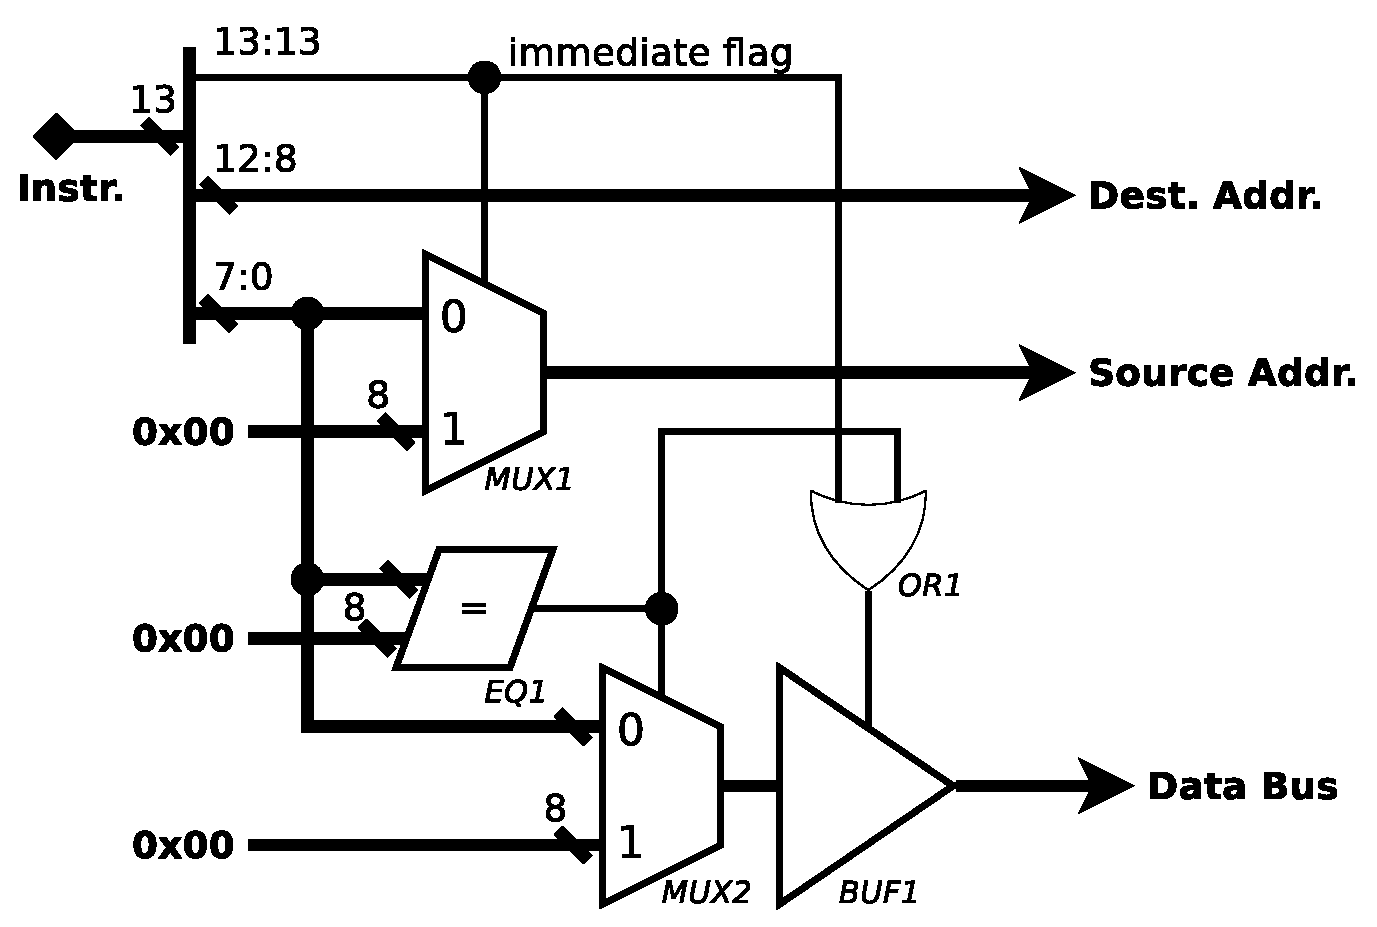
\includegraphics[scale=0.4]{../resources/oisc_decoder.eps}
	\caption{Digital diagram of OISC instruction decoder}
	\label{fig:oisc_decoder}
\end{figure*}

\subsection{Assembly}\label{subsec:assembly}
There are two steps between the assembly code and its execution on a processor. First, it needs to be converted into a binary machine code. Secondly, binary data needs to be sliced to different parts described in section \ref{subsec:memory}. These slices also need to be converted into appropriate formats, different for simulation, HDL synthesis and direct memory flashing. 

A universal assembler was implemented using python for both processors. The flowchart in figure \ref{fig:assembler} represents general structure of assembler process. It splits assembly file into three parts — sections, definitions and macros. Definitions are keywords mapped to values which are saved in a global label dictionary. Macros are a chunk of assembly code and are used as templates. 

There are only two sections implemented in assembler - \texttt{.text} and \texttt{.data}. Section \texttt{.text} contains all machine instructions which will be stored in program ROM memory. Section \texttt{.data} is used for global and static data, and it will be written into RAM memory. This section is used to store values such as strings and uninitialised data structures. These values are accessed with labels which correspond to RAM memory location. 

Section \texttt{.text} code is processed line by line. Each line may have label and an instruction or macro name following with argument values. If line contains a label, it is stored into global label dictionary with current line program address as a value. If line has a macro, line is replaces by macro code. Otherwise, instruction name is decoded and stored in an instruction list with original arguments.

After all instruction lines are completed, each stored instruction arguments are processed, labels are replaced with binary values, any other processing is done such as addition by constant, byte selection, etc. Completed list is then saved as a raw binary. Similarly, \texttt{.data} section labels also replaced and it is saved as binary data.

\begin{colfigure}
	\centering
	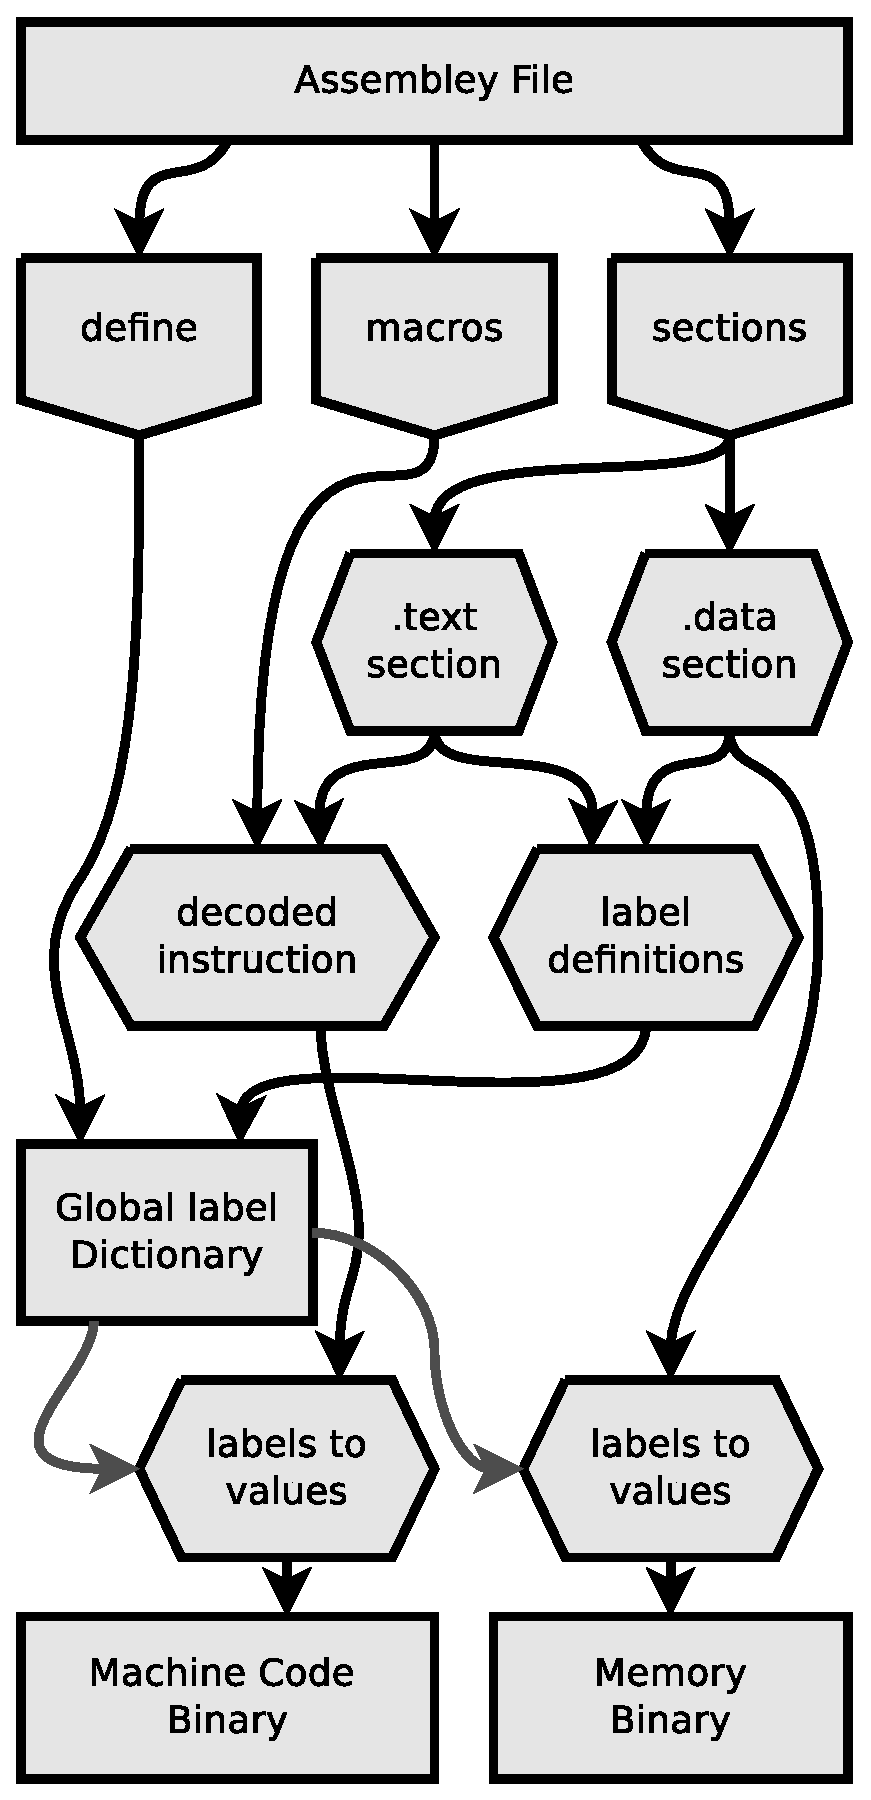
\includegraphics[scale=0.4]{../resources/assembler.eps}
	\captionof{figure}{Flow chart of assember converting assembly code into machine code and memory binary.}
	\label{fig:assembler}
\end{colfigure}

\subsection{System setup}\label{subsec:setup}
This section will describe how the system is set up.

Processors are implemented on Terasic DE0-Nano board that use Altera Cyclone IV, EP4CE22P17C6 FPGA, which is manufactured using $60nm$ fabrication technology.
The FPGA has embedded memory structure consisting of M9K memory blocks columns mentioned in Subsection \ref{subsec:oisc_mem}. These memory structures were used to implement processors RAM and ROM memories. Board also has 32MB SDRAM chip, which initially was intended to be used. This set design criteria to have 24bit address space. However, M9K memory was used instead for flexibility and simplicity. 

Thas FPGA has also an embedded phase-locked loop (PLL) stucture that is used to change 50MHz input that is generated by on-board crystal to other frequencies. 

DE0-Nano board has an integrated JTAG port that is used to upload synthesised code and control additional debugging tools. Quartus has a "Signal Tap Logic Analyzer" tool that allow setup probes and sources within FPGA logic and control them via JTAG. Another "In-System Memory Content Editor" tool allows read and modify M9K memory which enables quick machine code uploading to the processor on FPGA, without need to resynthesise HDL code. This also allow reading RAM content enabling easier program debugging. 

All Quartus functions can be accessed via TCL script. This lead to constructing Makefile which allow quick build operations. Quratus signal and memory tools were used to write a small program with Python and Curses library to read and change internal processor state which allowed easy debugging while writing the programs. 



	\vfill\pagebreak
	\section{Results and Analysis}\label{sec:results}
	\iffalse
This chapter looks specifically at your results.
* You measured some samples. 
What values did you measure? 
Present them in a table or graph? 
How did you test whether they were good measurements? 
Were you looking to improve something? 
Are your new samples better than the old ones?

* You built a device; 
what tests did you run to make sure that it is running correctly?

* You calculated something or developed a new theory about something. 
How do you know how well it predicts? 
What tests did you run? 
What comparisons with the literature did you make?
* You coded or simulated something. 
What tests did you run to be sure it was working correctly? 

Describe what you want the reader to notice in the results. 
Give the facts, then give your analysis of the facts.
Present your graphs, figures, tables, photos, and equations needed to show what you accomplished.
Label everything clearly, using the recommendations given below in “Things to Look For”
\fi

\subsection{Benchmark Programs}



\subsubsection{Number of instructions}

\subsubsection{Instruction composition}
Function composition was executed with following code:

\begin{lstlisting}[frame=single, caption={RISC assembly frame for executring tests}, emph={setup,start,done}]
setup:
	JUMP .start
.done:
	JUMP .done
.start:
	; Setup values
	; Call function
	JUMP .done
\end{lstlisting}

\begin{lstlisting}[frame=single, caption={OISC assembly frame for executring tests}, emph={setup,start,done}]
setup:
	BR1 .start @1
	BR0 .start @0
	BRZ 0x00
.done:
	BRZ 0x00
.start:
	; Setup values
	; Call function
	BR1 .done @1
	BR0 .done @0
	BRZ 0x00
\end{lstlisting}



\subsection{Maximum clock frequency}

\subsection{}


	\section{Conclusion}\label{sec:conclusion}
	% !TeX root = index.tex
\iffalse
The final chapter is short and sweet, to the point:
 what did you really accomplish? 
 What significant result can you claim and how it differs from anything done before. 
 How well did you meet your goal? 
 Now step out one level, then another indicating the impact your work will have on the literature and on future endeavours.
 * Start with the specifics and end with the general.
 * Summarise key result; mention limitations, note anything unexpected.
\fi

In this paper, two novel RISC and OISC-MOVE architectures were designed and implemented on a FPGA. Logic element requirements, power consumption, maximum frequency were tested. Benchmark programs execution times were used to compare these two processors and investigate OISC-MOVE advantages. It was shown that power consumption differences are insignificant, RISC managed to reach 40\% higher maximum frequency at 75-70MHz, however due to a timing design issue with OISC. OISC required 51.7\% less logic elements to implement on FPGA. Benchmarks showed that OISC took 71\% longer to execute on average while requiring 41.71\% more instruction space. 

This project has sucessfully covered its goals in studying architectures and investigating an alternative OISC implementation. Results show that proposed implementation of OISC-MOVE may be only suitable for microprocessor application with very strict logic element limit. 

RISC processor has been shown to be superior in tests, however it has more optimised implementation. Further research is needed to investigate OISC-MOVE performance with multiple data and instruction buses to match RISC complexity. 

	\vfill\pagebreak
	\printbibliography
	\onecolumn
	\section{Appendix}\label{sec:appendix}
	% !TeX root = index.tex

\subsection{Processor instruction set tables}\label{subsec:instruction_sets}
\arrayrulecolor{black}
\begin{longtable}[h!]{| l | p{.70\textwidth} | c |}
\caption{Instruction set for RISC processor. * Required immediate size in bytes}
\label{tab:risc_instructions}\\

\hline
\rowcolor[rgb]{0.82,0.82,0.82}
Instr. & Description & I-size *\\\hline
\endhead		

\arrayrulecolor{black}\hline
\endfoot

\multicolumn{3}{|c|}{
	\cellcolor[rgb]{0.7,0.7,1}\textit{2 register instructions}} \\\hline
\arrayrulecolor[rgb]{0.82,0.82,0.82}

MOVE & Copy value from one register to other & 0 \\\hline
ADD  & Arithmetical addition & 0 \\
SUB  & Arithmetical subtraction & 0  \\
AND  & Logical AND & 0 \\
OR   & Logical OR & 0 \\
XOR  & Logical XOR & 0 \\
MUL  & Arithmetical multiplication & 0 \\
DIV  & Arithmetical division (inc. modulus) & 0 \\


\arrayrulecolor{black}\hline
\multicolumn{3}{|c|}{
	\cellcolor[rgb]{0.7,0.7,1}\textit{1 register instructions}} \\
\hline\arrayrulecolor[rgb]{0.82,0.82,0.82}


COPY0 & Copy intimidate to a register 0 & 1 \\
COPY1 & Copy intimidate to a register 1 & 1 \\
COPY2 & Copy intimidate to a register 2 & 1 \\
COPY3 & Copy intimidate to a register 3 & 1 \\\hline

ADDC & Arithmetical addition with carry bit& 0 \\
ADDI & Arithmetical addition with immediate & 1 \\
SUBC & Arithmetical subtraction with carry bit & 0 \\
SUBI & Arithmetical subtraction with immediate & 1 \\\hline

ANDI & Logical AND with immediate & 1 \\
ORI  &  Logical OR with immediate & 1 \\
XORI &  Logical XOR with immediate & 1 \\\hline

CI0  & Replace intimidate value byte 0 for next instruction & 1 \\
CI1  & Replace intimidate value byte 1 for next instruction & 1 \\
CI2  & Replace intimidate value byte 2 for next instruction & 1 \\\hline

SLL  & Shift left logical & 1 \\
SRL  & Shift right logical & 1 \\
SRA  & Shift right arithmetical & 1 \\\hline

LWHI & Load word (high byte) & 3 \\
SWHI & Store word (high byte, reg. only) & 0 \\
LWLO & Load word (low byte) & 3 \\
SWLO & Store word (low byte, stores high byte reg.) & 3 \\\hline

INC  & Increase by 1 & 0 \\
DEC  & Decrease by 1 & 0 \\
GETAH& Get ALU high byte reg. (only for MUL \& DIV \& ROL \& ROR) & 0 \\
GETIF& Get interrupt flags & 0 \\\hline

PUSH & Push to stack & 0 \\
POP  & Pop from stack & 0 \\
COM  & Send/Receive to/from com. block & 1 \\\hline

BEQ  & Branch on equal & 3 \\
BGT  & Branch on greater than & 3 \\
BGE  & Branch on greater equal than & 3 \\
BZ   & Branch on zero & 2 \\

\arrayrulecolor{black}\hline
\multicolumn{3}{|c|}{
	\cellcolor[rgb]{0.7,0.7,1}\textit{0 register instructions}
} \\
\hline\arrayrulecolor[rgb]{0.82,0.82,0.82} 

CALL & Call function, put return to stack & 2 \\
RET  & Return from function & 0 \\
JUMP & Jump to address & 2 \\
RETI & Return from interrupt & 0 \\
INTRE& Set interrupt entry pointer & 2 \\\hline


\end{longtable}	

\arrayrulecolor{black}
\begin{longtable}[h!]{| l | p{0.8\textwidth} |}
	\caption{Instructions for OISC processor.}
	\label{tab:oisc_instructions}\\
	
	\hline 
	\rowcolor[rgb]{0.82,0.82,0.82}
	Name & Description \\\hline
	\endhead		
	
	\arrayrulecolor{black}\hline
	\endfoot
	
	\multicolumn{2}{|c|}{
		\cellcolor[rgb]{0.7,0.7,1}\textit{Destination Addresses}} \\\hline
	\arrayrulecolor[rgb]{0.82,0.82,0.82}
	
	ACC0 & Set ALU source A accumulator \\
	ACC1 & Set ALU source B accumulator \\\hline
	BR0  & Set Branch pointer register (low byte) \\
	BR1  & Set Branch pointer register (high byte) \\
	BRZ  & If source value is 0, set program counter to branch pointer \\\hline
	STACK& Push value to stack \\
	MEM0 & Set Memory pointer register (low byte) \\
	MEM1 & Set Memory pointer register (middle byte) \\
	MEM2 & Set Memory pointer register (high byte) \\
	MEMHI& Save high byte to memory at memory pointer \\
	MEMLO& Save low byte to memory at memory pointer \\\hline
	COMA & Set communication block address register \\
	COMD & Send value to communication block \\\hline
	REG0 & Set general purpose register 0 \\
	REG1 & set general purpose register 1 \\
	
	\arrayrulecolor{black}\hline
	\multicolumn{2}{|c|}{
		\cellcolor[rgb]{0.7,0.7,1}\textit{Source Addresses}} \\\hline
	\arrayrulecolor[rgb]{0.82,0.82,0.82}
	
	NULL & Get constant 0 \\
	ALU0 & Get value at ALU source A accumulator \\
	ALU1 & Get value at ALU source B accumulator \\\hline
	
	ADD  & Get Arithmetical addition of ALU sources \\
	ADDC & Get Arithmetical addition carry \\
	ADC  & Get Arithmetical addition of ALU sources and carry \\\hline
	
	SUB  & Get Arithmetical subtraction of ALU sources \\
	SUBC & Get Arithmetical subtraction carry \\
	SBC  & Get Arithmetical subtraction of ALU sources and carry \\\hline
	
	AND  & Get Logical AND of ALU sources \\
	OR   & Get Logical OR of ALU sources \\
	XOR  & Get Logical XOR of ALU sources \\\hline
	
	SLL  & Get ALU source A shifted left by source B \\
	SRL  & Get ALU source A shifted right by source B \\
	ROL  & Get rolled off value from previous SLL instance \\
	ROR  & Get rolled off value from previous SRL instance \\\hline
	
	MULLO& Get Arithmetical multiplication of ALU sources (low byte) \\
	MULHI& Get Arithmetical multiplication of ALU sources (high byte) \\
	DIV  & Get Arithmetical division of ALU sources \\
	MOD  & Get Arithmetical modulus of ALU sources \\\hline
	
	EQ   & Check if ALU source A is equal to source B \\
	GT   & Check if ALU source A is greater than source B \\
	GE   & Check if ALU source A is greater or equal to source B \\
	NE   & Check if ALU source A is not equal to source B \\
	LT   & Check if ALU source A is less than source B \\
	LE   & Check if ALU source A is less or equal to to source B \\\hline
	
	BR0  & Get Branch pointer register value (low byte) \\
	BR1  & Get Branch pointer register value (high byte) \\	
	PC0  & Get Program counter value (low byte) \\
	PC1  & Get Program counter value (high byte) \\\hline
	
	MEM0 & Get Memory pointer register value (low byte) \\
	MEM1 & Get Memory pointer register value (middle byte) \\
	MEM2 & Get Memory pointer register value (high byte) \\
	MEMHI& Load high byte from memory at memory pointer \\
	MEMLO& Load low byte from memory at memory pointer \\\hline
	
	STACK& Pop value from stack \\
	ST0  & Get stack address value (low byte) \\
	ST1  & Get stack address value (high byte) \\
	
	COMA & Get communication block address register value \\
	COMD & Read value from communication block \\\hline
	
	REG0 & Get value from general purpose register 0 \\
	REG1 & Get value from general purpose register 1 \\
	
\end{longtable}	
	
\end{document}